\chapter{La détection des anomalies dans les délais d'un lien} \label{chap:algorith-detection}

Dans le présent chapitre, nous présentons l'outil de détection des anomalies dans les délais d'un lien  conçu dans le cadre de l'étude  de  Fontugne et al. \cite{DBLP:journals/corr/FontugneAPB16}. Nous avons choisi ce travail qui exploite des données massives en vue d'évaluer quelques technologies  Big Data.

\section{Introduction}
Le travail de  Fontugne  et al.\cite{DBLP:journals/corr/FontugneAPB16} exploite une des mesures effectuées par les sondes Atlas: la requête traceroute. L'idée de ce travail est de collecter les résultats des requêtes traceroute effectuées par les sondes Atlas, d'en déterminer une valeur de référence sur base de l'historique, et ensuite de comparer la référence avec la valeur courante. La référence pour le délai  d'un lien donné   est mise à jour au fur et à mesure de l'analyse.



Dans leur travail \cite{DBLP:journals/corr/FontugneAPB16}, Fontugne et al. ont exploité la  distribution répandue des sondes Atlas dans le monde afin d'étudier un des problèmes relatifs aux performances des réseaux informatiques. 

En pratique, il est  difficile  d'avoir une idée globale et exacte sur la topologie d'Internet. Toutefois, les opérateurs des réseaux informatiques  disposent d'un aperçu de l'état des entités qui forment leurs réseaux, les relations entre ces entités ainsi que les éventuels problèmes. Avec la distribution abondante des sondes Atlas dans le monde en terme de type d'adressage : sondes Atlas supportant seulement l'adressage IPv4, d'autres qui supportent en plus l'adressage IPv6, en terme de  la diversité géographique, la diversité en terme d'ASs hébergeant les sondes Atlas, etc, il était  possible d'aborder  les délais dans les réseaux informatiques à travers de nouvelles approches, reposées sur des fondements statistiques. Parmi les points forts de l'analyse menée par  Fontugne et al., c'était la possibilité de valider les   méthodes proposées avec des événements  marquants sur Internet.

Le travail de R. Fontugne et al. reprend trois méthodes basées sur les données collectées par les sondes Atlas :

\begin{enumerate}
	\item la détection des changements des délais que subissent les liens intermédiaires dans les traceroutes; 
	
	\item la conception d'un modèle de forwording pour un routeur donné. Ce modèle  prédit l'acheminement du trafic afin d'identifier les routeurs  et les liens en panne dans le cas  d'un problème  de perte de paquets;
	
	\item la création d'un score par Système Autonome afin d'évaluer l'état de ce dernier.
	
\end{enumerate}

Dans la suite de ce travail, nous  reprendrons seulement la première méthode.  Il s'agit d'étudier le délai d'un lien topologique; c'est le délai entre deux routeurs adjacents sur Internet. Nous aurions aimé avoir suffisamment de temps pour pouvoir aborder les autres méthodes.  



\section{Pourquoi analyser les délais des liens réseaux}

Il existe un bon nombre de sujets à traiter en exploitant les données collectées par les sondes Atlas. Quelques exemples de sujets ont été déjà présentés dans la section \ref{use-cases-atlas}. Notre choix de reprendre le travail de Fontugne et al. a été fait après avoir parcouru un ensemble de travaux basés sur le projet  RIPE Atlas. 

Pour certains travaux, il n'était pas possible  de les reprendre suite au manque de détails et de l'accès à  certaines ressources réseaux utilisées dans ces travaux \footnote{Par exemple, les informations du peering entre les Systèmes Autonomes, la géolocalisation des adresses IP, etc.}. Par exemple, afin d'étudier la censure dans un pays donné, il faut être au courant des spécificités de ce pays, les circonstances politiques et sociales, les opposants,  etc.  Un autre exemple concerne le sujet de la détection des détours du trafic local dans un pays.  Anant Shah  et al. ont travaillé sur la détection des détours \cite{anant-shah} où ils ont présenté  les contraintes relatives à ce sujet: la difficulté d'avoir une géolocalisation exacte d'une adresse IP d'une part et l'absence des informations de peering entre les ASs d'autre part. Ces dernières peuvent changer complètement les conclusions finales. 

Le travail sur lequel nous nous basons \cite{DBLP:journals/corr/FontugneAPB16} s'inscrit dans les travaux traitant les performances des réseaux. Dans la suite de ce document, ce travail sera utilisé comme travail de référence.  Ce travail a été choisi comme référence pour plusieurs raisons:


	
\paragraph{Les données utilisées}  Les auteurs de ce travail ont exploité des données déjà présentes dans la base de données du RIPE Atlas. Ainsi, il n'y a pas besoin de lancer des mesures qui nécessitent la possession d'assez de crédits \footnote{Voir la section \ref{credits-atlas}.}. De plus, les mesures intégrées montrent plus de stabilité par rapport aux mesures personnalisées. Les destinations des mesures intégrées sont prédéfinies, généralement ce sont des instances des serveurs DNS et des serveurs gérés par  RIPE NCC. Cependant, les mesures personnalisées peuvent concerner des destinations moins stables en terme de disponibilité.
	
\paragraph{La clarté du travail} La communauté RIPE Atlas est active en nombre de travaux publiés. Cependant, ces travaux reprennent seulement les résultats. Pour certains,  la méthodologie a été bien détaillée. Pour d'autres, la méthodologie adoptée était très brève. En ce qui concerne le  travail choisi, il  est bien détaillé.
	
\paragraph{La disponibilité du code source} La détection des anomalies proposée a été mise en pratique à travers un outil. Les code source de cet outil est disponible sur GitHub\cite{InternetHealthReport}. L'accès au code source de l'outil nous a permis de bien comprendre la démarche de la détection.

%Avoir le code source disponible sur GitHub est avantageux. L'objectif n'était pas de réécrire ce que les auteurs ont fait, mais plutôt le comprendre et éventuellement l'ajuster suivant les besoins.  De plus, l'onglet \textit{issues} du projet permet de  demander des détails aux contributeurs mais aussi cela permet de partager les réflexions.
	
\paragraph{La possibilité de la validation des résultats}  Comme il était cité dans le travail \cite{DBLP:journals/corr/FontugneAPB16}, les auteurs ont démontré la cohérence de l'outil de détection avec des éventements réels comme les  attaques DDOS.
	
	\begin{tcolorbox}
		Une attaque de type Distributed Denial of Service (\textbf{\textit{DDOS}}) vise la disponibilité d'un serveur en surchargeant ce dernier avec un trafic depuis différentes sources, d'où le terme \textit{Distributed}.
	\end{tcolorbox}
	

\section{L'étude des délais des liens } 

\subsection{Les données utilisées dans l'analyse des délais}~

La méthode conçue pour la détection des changements des délais se base sur des fondements statistiques. Ces derniers sont capables de montrer leurs performances si la taille des échantillons \footnote{L'échantillon de la métrique qui caractérise un lien : RTT différentiel.} considérés est grande.   Afin de surveiller un grand nombre de liens sur Internet, il faut avoir un grand nombre de sondes Atlas avec une certaine diversité.

Le travail de référence implique principalement les mesures de traceroutes. On distingue  deux catégories de mesures  utilisées :

\begin{itemize}
	\item \textit{builtin} : ce sont les traceroutes effectués par toutes les sondes Atlas vers les instances des  $13$ serveurs DNS racines. Les traceroutes sont effectués chaque $30$ minutes. En pratique, certains serveurs racines DNS déploient l'anycast. Au moment de la réalisation du travail de référence\footnote{Année $2017$.}, c'étaient des traceroutes vers $ 500 $ instances des serveurs DNS racines;
	\begin{tcolorbox}
		\textbf{DNS Anycast} est une solution   utilisée pour accélérer le fonctionnement  des serveurs DNS. Les serveurs DNS adoptant cette approche fournissent des temps de réponse plus courts, et ce partout dans le monde. Les requêtes en provenance de l'utilisateur sont redirigées vers un n\oe{}ud adéquat suivant un algorithme prédéfini. 
	\end{tcolorbox}
	
	\item \textit{anchoring} : ce sont les traceroutes effectués par environ $400$ sondes Atlas à destination de $189$ serveurs\footnote{Sondes Atlas ayant des fonctionnalités avancées.} et ce chaque $15$ minutes.
\end{itemize}

En ce qui concerne le nombre de  traceroutes analysés, le tableau \ref{tab:dataset} reprend plus de détails; le nombre de traceroutes ainsi que le nombre de sondes impliquées dans ces traceroutes, pour les deux types d'adressages (IPv4 et IPv6). 

\begin{table}[H]
	\centering
	\begin{tabular}{|l|l|l|}
		\hline
		& \textbf{Nombre de traceroute}s& \textbf{Nombre de sondes}\\ \hline
		IPv4		&$ 2.8 $ milliards & $ 11,538 $\\ \hline
		IPv6	&	$ 1.2 $ milliards & $ 4,30 $ \\ \hline
	\end{tabular}
	\caption{Récapitulatif des traceroutes utilisés dans le travail de référence }
	\label{tab:dataset}
\end{table}


Pour précision, l'étude des délais des liens ne concerne pas  les adresses privées, ainsi, le suivi des délais ne concerne pas les réseaux privés.  De plus, ce  suivi  se base sur les requêtes de type traceroute, et traceroute reprend une partie de la topologie de l'Internet. En effet, les liens considérés sont ceux topologiques et ne sont pas  les liens physiques. 

\subsection{Le principe de la détection des changements des délais} \label{principe-de-detection}
\paragraph{Définition du RTT différentiel }~

Avant de définir le RTT différentiel, soit la définition du RTT :
%Il est indispensable de présenter la définition du RTT  (Round Trip Time)  différentiel d'un lien avant de procéder à la description de l'algorithme de la détection des anomalies. 


\begin{tcolorbox}
	
	\textbf{ICMP} (Internet Control Message Protocol) est un protocole utilisé pour véhiculer des messages de contrôle sur Internet.
	
	\textbf{RTT} est obtenu en calculant la différence entre le timestamp associé à l'envoi du paquet vers une destination  et le timestamp associé à la réception de la réponse ICMP de cette destination. C'est une métrique pour évaluer les performances d'un réseau en matière de temps de réponse. Les mesures du RTT sont fournies par les utilitaires traceroute et ping. En ce qui concerne traceroute,  ce dernier fournit les sauts impliqués dans le  chemin de forwarding, c'est le chemin parcouru par le trafic entre la source et la destination.  RTT inclut le temps de transmission, du quering et  du traitement. 
\end{tcolorbox}

La figure 	\ref{fig:rtt-differ} (a)  illustre le RTT entre la sonde P  deux routeurs B et C. Le RTT différentiel   $B$ et $C$ adjacents, noté $\Delta_{PBC}$, est la différence du RTT entre la sonde $P$ et $B$ (bleu) d'une part, et du RTT entre la sonde $P$ et $C$ (rouge) dans la figure 	\ref{fig:rtt-differ} (b). 

\begin{align*}
\Delta_{PBC} &= RTT_{PC} - RTT_{PB} \\
&= \delta_{BC} + \delta_{CD} + \delta_{DA}  - \delta_{BA} \\
&= \delta_{BC} + \varepsilon_{PBC}
\end{align*}

où $\delta_{BC}$ est le délai du lien $BC$ et $\varepsilon_{PBC}$ est la différence entre les deux chemins de retour ($B$ vers $P$ et $C$ vers $P$). 
%La première composante dépend de l'état des routeurs $B$ et $C$. La deuxième composante dépend de la sonde $P$. L'analyse du RTT différentiel repose sur la variation de valeurs qu'il prend, au lieu des valeurs exactes, dans  le cas des valeurs exactes, elles peuvent dévier l'interprétation.
\begin{figure}[H]
	\centering
		\captionsetup{justification= centering}
	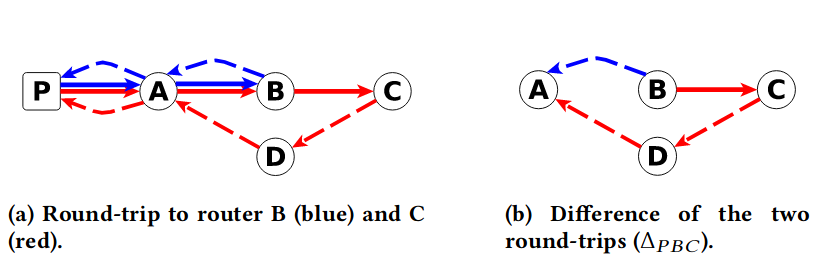
\includegraphics[width=0.7\linewidth]{illustrations/rtt-differ}
	\caption{(a) Le RTT entre la sonde P et les routeurs B et C. (b) La différence entre les  chemins de retour depuis les routeurs B et C vers la sonde P. Source : \cite{DBLP:journals/corr/FontugneAPB16}}
	\label{fig:rtt-differ}
\end{figure}

\paragraph{Le principe de la détection des changements des délais}

L'évolution du délai d'un lien est déduit de l'évolution de son RTT différentiel. Reprenons d'abord la formule du RTT différentiel du lien BC : 

 $\delta_{BC}$ + $\varepsilon_{PBC}$. 
 
 Supposons qu'on dispose d'un nombre $n$ de sondes Atlas P$_i$, $i$ $\in$ [$1$, $n$], telles que toutes les sondes ont un chemin de retour différent depuis B et depuis C.  En effet, les RTTs différentiels pour chacune des sondes Atlas $\Delta_{P{_i}BC}$ partagent la même composante $\delta_{BC}$.

On sait que les $n$ sondes Atlas sont indépendantes; le chemin de retour de chacune est indépendant, ainsi les valeurs des  $\varepsilon_{P_{i}BC}$ sont  indépendantes. L'indépendance de ces valeurs implique que la distribution $\Delta_{P_{i}BC}$ est estimé  stable au cours du temps si $\delta_{BC}$ est constant. Cependant, un changement significatif de la valeur de $\delta_{BC}$ influence les valeurs des RTTs différentiels. Dans ce cas, la distribution des RTTs différentiels change. 

%Enfin, les changements des délais sont déduits des changements des RTTs différentiel qu'on peut les quantifier.

La détection des anomalies des délais repose sur le théorème  central limite (TCL). Ce théorème  annonce que si on a une suite de variables aléatoires $X_i$ indépendantes ayant la même espérance $\mu$ et la même variance $\sigma^2$, la moyenne de ces variables aléatoires est une variable aléatoire qui suit une loi normale. 

%De manière générale, le théorème central limite explique la distribution des moyennes des échantillons. Ce théorème peut être appliquer aux différents lois. Par exemple la loi normale \footnote{Un exemple illustratif dans \ref{appendix:clt-exemple}.}, binomiale, etc. 



\section{L'évolution du RTT différentiel des liens}

L'évolution des RTTs différentiels est une des applications du principe décrit dans  \ref{principe-de-detection}. Pour un lien donné, le suivi est fait sur plusieurs  périodes. En plus du suivi du RTT différentiel, il y a aussi l'identification d'éventuelles anomalies pour ce lien.

\subsection{Description des paramètres de l'analyse des délais} \label{par:parametre-de-lanalyse}~

La détection des changements des délais nécessite l'ajustement d'un nombre de paramètres. La valeur de chaque paramètre est relative au  fondement utilisé théorique ou bien empirique, qui a été  justifié par les auteurs du travail de référence.   Ci-dessous les paramètres à ajuster afin d'obtenir l'évolution des RTTs différentiels d'un lien ainsi que les éventuelles anomalies.  

\textbf{start} : c'est la date de début de l'analyse. Seuls les traceroutes effectués par les sondes Atlas à partir de cette date qui sont analysés.

\textbf{end} : c'est la date marquant la fin de l'analyse. Comme le paramètre \textit{start}, c'est la date maximales des  traceroutes effectués par les sondes Atlas à considérer.

\textbf{timeWindow} :  ce paramètre est exprimé en secondes. Il correspond à la durée des périodes de l'analyse. Ces périodes ont la même durée. Autrement dit, la durée entre   \textit{start} et \textit{end} est divisée sur
 cette même taille: \textit{timeWindow}, c'est qui est illustré dans la Figure  \ref{fig:timing_tex}.

%illustre le contexte des trois paramètres \textit{start}, \textit{end} et \textit{timeWindow} avec les étapes principales.



\begin{figure}[h]
	\centering
	\captionsetup{justification=centering}
	% Graphic for TeX using PGF
% Title: /home/hayat/RipeAtlasTraceroutesAnalysis/report/illustrations/timing.dia
% Creator: Dia v0.97+git
% CreationDate: Mon Dec  3 23:19:01 2018
% For: hayat
% \usepackage{tikz}
% The following commands are not supported in PSTricks at present
% We define them conditionally, so when they are implemented,
% this pgf file will use them.
\ifx\du\undefined
  \newlength{\du}
\fi
\setlength{\du}{15\unitlength}
\begin{tikzpicture}[even odd rule]
\pgftransformxscale{1.000000}
\pgftransformyscale{-1.000000}
\definecolor{dialinecolor}{rgb}{0.000000, 0.000000, 0.000000}
\pgfsetstrokecolor{dialinecolor}
\pgfsetstrokeopacity{1.000000}
\definecolor{diafillcolor}{rgb}{1.000000, 1.000000, 1.000000}
\pgfsetfillcolor{diafillcolor}
\pgfsetfillopacity{1.000000}
\pgfsetlinewidth{0.100000\du}
\pgfsetdash{}{0pt}
\pgfsetbuttcap
{
\definecolor{diafillcolor}{rgb}{0.000000, 0.000000, 0.000000}
\pgfsetfillcolor{diafillcolor}
\pgfsetfillopacity{1.000000}
% was here!!!
}
\definecolor{dialinecolor}{rgb}{0.000000, 0.000000, 0.000000}
\pgfsetstrokecolor{dialinecolor}
\pgfsetstrokeopacity{1.000000}
\draw (34.600000\du,6.050000\du)--(40.550000\du,6.000000\du);
\pgfsetlinewidth{0.100000\du}
\pgfsetdash{}{0pt}
\pgfsetmiterjoin
\pgfsetbuttcap
\definecolor{dialinecolor}{rgb}{0.000000, 0.000000, 0.000000}
\pgfsetstrokecolor{dialinecolor}
\pgfsetstrokeopacity{1.000000}
\draw (35.097882\du,5.795807\du)--(35.102083\du,6.295790\du);
\pgfsetlinewidth{0.100000\du}
\pgfsetdash{}{0pt}
\pgfsetmiterjoin
\pgfsetbuttcap
\definecolor{dialinecolor}{rgb}{0.000000, 0.000000, 0.000000}
\pgfsetstrokecolor{dialinecolor}
\pgfsetstrokeopacity{1.000000}
\draw (40.052118\du,6.254193\du)--(40.047917\du,5.754210\du);
% setfont left to latex
\definecolor{dialinecolor}{rgb}{0.000000, 0.000000, 0.000000}
\pgfsetstrokecolor{dialinecolor}
\pgfsetstrokeopacity{1.000000}
\definecolor{diafillcolor}{rgb}{0.000000, 0.000000, 0.000000}
\pgfsetfillcolor{diafillcolor}
\pgfsetfillopacity{1.000000}
\node[anchor=base west,inner sep=0pt,outer sep=0pt,color=dialinecolor] at (14.800200\du,8.464650\du){start};
% setfont left to latex
\definecolor{dialinecolor}{rgb}{0.000000, 0.000000, 0.000000}
\pgfsetstrokecolor{dialinecolor}
\pgfsetstrokeopacity{1.000000}
\definecolor{diafillcolor}{rgb}{0.000000, 0.000000, 0.000000}
\pgfsetfillcolor{diafillcolor}
\pgfsetfillopacity{1.000000}
\node[anchor=base west,inner sep=0pt,outer sep=0pt,color=dialinecolor] at (39.375600\du,7.990890\du){end};
% setfont left to latex
\definecolor{dialinecolor}{rgb}{0.000000, 0.000000, 0.000000}
\pgfsetstrokecolor{dialinecolor}
\pgfsetstrokeopacity{1.000000}
\definecolor{diafillcolor}{rgb}{0.000000, 0.000000, 0.000000}
\pgfsetfillcolor{diafillcolor}
\pgfsetfillopacity{1.000000}
\node[anchor=base west,inner sep=0pt,outer sep=0pt,color=dialinecolor] at (24.374800\du,8.977310\du){Périodes de l'analyse};
% setfont left to latex
\definecolor{dialinecolor}{rgb}{0.000000, 0.000000, 0.000000}
\pgfsetstrokecolor{dialinecolor}
\pgfsetstrokeopacity{1.000000}
\definecolor{diafillcolor}{rgb}{0.000000, 0.000000, 0.000000}
\pgfsetfillcolor{diafillcolor}
\pgfsetfillopacity{1.000000}
\node[anchor=base west,inner sep=0pt,outer sep=0pt,color=dialinecolor] at (14.950000\du,7.200000\du){d1};
\pgfsetlinewidth{0.100000\du}
\pgfsetdash{}{0pt}
\pgfsetbuttcap
{
\definecolor{diafillcolor}{rgb}{0.000000, 0.000000, 0.000000}
\pgfsetfillcolor{diafillcolor}
\pgfsetfillopacity{1.000000}
% was here!!!
}
\definecolor{dialinecolor}{rgb}{0.000000, 0.000000, 0.000000}
\pgfsetstrokecolor{dialinecolor}
\pgfsetstrokeopacity{1.000000}
\draw (29.656800\du,6.066270\du)--(35.606800\du,6.016270\du);
\pgfsetlinewidth{0.100000\du}
\pgfsetdash{}{0pt}
\pgfsetmiterjoin
\pgfsetbuttcap
\definecolor{dialinecolor}{rgb}{0.000000, 0.000000, 0.000000}
\pgfsetstrokecolor{dialinecolor}
\pgfsetstrokeopacity{1.000000}
\draw (30.154682\du,5.812077\du)--(30.158883\du,6.312060\du);
\pgfsetlinewidth{0.100000\du}
\pgfsetdash{}{0pt}
\pgfsetmiterjoin
\pgfsetbuttcap
\definecolor{dialinecolor}{rgb}{0.000000, 0.000000, 0.000000}
\pgfsetstrokecolor{dialinecolor}
\pgfsetstrokeopacity{1.000000}
\draw (35.108918\du,6.270463\du)--(35.104717\du,5.770480\du);
\pgfsetlinewidth{0.100000\du}
\pgfsetdash{}{0pt}
\pgfsetbuttcap
{
\definecolor{diafillcolor}{rgb}{0.000000, 0.000000, 0.000000}
\pgfsetfillcolor{diafillcolor}
\pgfsetfillopacity{1.000000}
% was here!!!
}
\definecolor{dialinecolor}{rgb}{0.000000, 0.000000, 0.000000}
\pgfsetstrokecolor{dialinecolor}
\pgfsetstrokeopacity{1.000000}
\draw (24.701800\du,6.106100\du)--(30.651800\du,6.056100\du);
\pgfsetlinewidth{0.100000\du}
\pgfsetdash{}{0pt}
\pgfsetmiterjoin
\pgfsetbuttcap
\definecolor{dialinecolor}{rgb}{0.000000, 0.000000, 0.000000}
\pgfsetstrokecolor{dialinecolor}
\pgfsetstrokeopacity{1.000000}
\draw (25.199682\du,5.851907\du)--(25.203883\du,6.351890\du);
\pgfsetlinewidth{0.100000\du}
\pgfsetdash{}{0pt}
\pgfsetmiterjoin
\pgfsetbuttcap
\definecolor{dialinecolor}{rgb}{0.000000, 0.000000, 0.000000}
\pgfsetstrokecolor{dialinecolor}
\pgfsetstrokeopacity{1.000000}
\draw (30.153918\du,6.310293\du)--(30.149717\du,5.810310\du);
\pgfsetlinewidth{0.100000\du}
\pgfsetdash{}{0pt}
\pgfsetbuttcap
{
\definecolor{diafillcolor}{rgb}{0.000000, 0.000000, 0.000000}
\pgfsetfillcolor{diafillcolor}
\pgfsetfillopacity{1.000000}
% was here!!!
}
\definecolor{dialinecolor}{rgb}{0.000000, 0.000000, 0.000000}
\pgfsetstrokecolor{dialinecolor}
\pgfsetstrokeopacity{1.000000}
\draw (19.796600\du,6.121020\du)--(25.746600\du,6.071020\du);
\pgfsetlinewidth{0.100000\du}
\pgfsetdash{}{0pt}
\pgfsetmiterjoin
\pgfsetbuttcap
\definecolor{dialinecolor}{rgb}{0.000000, 0.000000, 0.000000}
\pgfsetstrokecolor{dialinecolor}
\pgfsetstrokeopacity{1.000000}
\draw (20.294482\du,5.866827\du)--(20.298683\du,6.366810\du);
\pgfsetlinewidth{0.100000\du}
\pgfsetdash{}{0pt}
\pgfsetmiterjoin
\pgfsetbuttcap
\definecolor{dialinecolor}{rgb}{0.000000, 0.000000, 0.000000}
\pgfsetstrokecolor{dialinecolor}
\pgfsetstrokeopacity{1.000000}
\draw (25.248718\du,6.325213\du)--(25.244517\du,5.825230\du);
\pgfsetlinewidth{0.100000\du}
\pgfsetdash{}{0pt}
\pgfsetbuttcap
{
\definecolor{diafillcolor}{rgb}{0.000000, 0.000000, 0.000000}
\pgfsetfillcolor{diafillcolor}
\pgfsetfillopacity{1.000000}
% was here!!!
}
\definecolor{dialinecolor}{rgb}{0.000000, 0.000000, 0.000000}
\pgfsetstrokecolor{dialinecolor}
\pgfsetstrokeopacity{1.000000}
\draw (14.841600\du,6.135940\du)--(20.791600\du,6.085940\du);
\pgfsetlinewidth{0.100000\du}
\pgfsetdash{}{0pt}
\pgfsetmiterjoin
\pgfsetbuttcap
\definecolor{dialinecolor}{rgb}{0.000000, 0.000000, 0.000000}
\pgfsetstrokecolor{dialinecolor}
\pgfsetstrokeopacity{1.000000}
\draw (15.339482\du,5.881747\du)--(15.343683\du,6.381730\du);
\pgfsetlinewidth{0.100000\du}
\pgfsetdash{}{0pt}
\pgfsetmiterjoin
\pgfsetbuttcap
\definecolor{dialinecolor}{rgb}{0.000000, 0.000000, 0.000000}
\pgfsetstrokecolor{dialinecolor}
\pgfsetstrokeopacity{1.000000}
\draw (20.293718\du,6.340133\du)--(20.289517\du,5.840150\du);
% setfont left to latex
\definecolor{dialinecolor}{rgb}{0.000000, 0.000000, 0.000000}
\pgfsetstrokecolor{dialinecolor}
\pgfsetstrokeopacity{1.000000}
\definecolor{diafillcolor}{rgb}{0.000000, 0.000000, 0.000000}
\pgfsetfillcolor{diafillcolor}
\pgfsetfillopacity{1.000000}
\node[anchor=base west,inner sep=0pt,outer sep=0pt,color=dialinecolor] at (19.845000\du,7.235000\du){d2};
% setfont left to latex
\definecolor{dialinecolor}{rgb}{0.000000, 0.000000, 0.000000}
\pgfsetstrokecolor{dialinecolor}
\pgfsetstrokeopacity{1.000000}
\definecolor{diafillcolor}{rgb}{0.000000, 0.000000, 0.000000}
\pgfsetfillcolor{diafillcolor}
\pgfsetfillopacity{1.000000}
\node[anchor=base west,inner sep=0pt,outer sep=0pt,color=dialinecolor] at (24.750000\du,7.300000\du){d3};
% setfont left to latex
\definecolor{dialinecolor}{rgb}{0.000000, 0.000000, 0.000000}
\pgfsetstrokecolor{dialinecolor}
\pgfsetstrokeopacity{1.000000}
\definecolor{diafillcolor}{rgb}{0.000000, 0.000000, 0.000000}
\pgfsetfillcolor{diafillcolor}
\pgfsetfillopacity{1.000000}
\node[anchor=base west,inner sep=0pt,outer sep=0pt,color=dialinecolor] at (29.740000\du,7.175000\du){di};
% setfont left to latex
\definecolor{dialinecolor}{rgb}{0.000000, 0.000000, 0.000000}
\pgfsetstrokecolor{dialinecolor}
\pgfsetstrokeopacity{1.000000}
\definecolor{diafillcolor}{rgb}{0.000000, 0.000000, 0.000000}
\pgfsetfillcolor{diafillcolor}
\pgfsetfillopacity{1.000000}
\node[anchor=base west,inner sep=0pt,outer sep=0pt,color=dialinecolor] at (34.685000\du,7.165000\du){di+1};
\pgfsetlinewidth{0.100000\du}
\pgfsetdash{}{0pt}
\pgfsetbuttcap
\definecolor{dialinecolor}{rgb}{0.000000, 0.000000, 0.000000}
\pgfsetstrokecolor{dialinecolor}
\pgfsetstrokeopacity{1.000000}
\pgfpathmoveto{\pgfpoint{25.180033\du}{4.900033\du}}
\pgfpatharc{315}{226}{3.501250\du and 3.501250\du}
\pgfusepath{stroke}
% setfont left to latex
\definecolor{dialinecolor}{rgb}{0.000000, 0.000000, 0.000000}
\pgfsetstrokecolor{dialinecolor}
\pgfsetstrokeopacity{1.000000}
\definecolor{diafillcolor}{rgb}{0.000000, 0.000000, 0.000000}
\pgfsetfillcolor{diafillcolor}
\pgfsetfillopacity{1.000000}
\node[anchor=base west,inner sep=0pt,outer sep=0pt,color=dialinecolor] at (20.780000\du,3.400000\du){timeWindow};
\pgfsetlinewidth{0.100000\du}
\pgfsetdash{}{0pt}
\pgfsetbuttcap
\definecolor{dialinecolor}{rgb}{0.000000, 0.000000, 0.000000}
\pgfsetstrokecolor{dialinecolor}
\pgfsetstrokeopacity{1.000000}
\pgfpathmoveto{\pgfpoint{29.975033\du}{4.885033\du}}
\pgfpatharc{315}{226}{3.501250\du and 3.501250\du}
\pgfusepath{stroke}
% setfont left to latex
\definecolor{dialinecolor}{rgb}{0.000000, 0.000000, 0.000000}
\pgfsetstrokecolor{dialinecolor}
\pgfsetstrokeopacity{1.000000}
\definecolor{diafillcolor}{rgb}{0.000000, 0.000000, 0.000000}
\pgfsetfillcolor{diafillcolor}
\pgfsetfillopacity{1.000000}
\node[anchor=base west,inner sep=0pt,outer sep=0pt,color=dialinecolor] at (25.675000\du,3.485000\du){timeWindow};
\pgfsetlinewidth{0.100000\du}
\pgfsetdash{}{0pt}
\pgfsetbuttcap
\definecolor{dialinecolor}{rgb}{0.000000, 0.000000, 0.000000}
\pgfsetstrokecolor{dialinecolor}
\pgfsetstrokeopacity{1.000000}
\pgfpathmoveto{\pgfpoint{20.275033\du}{4.785033\du}}
\pgfpatharc{315}{226}{3.501250\du and 3.501250\du}
\pgfusepath{stroke}
% setfont left to latex
\definecolor{dialinecolor}{rgb}{0.000000, 0.000000, 0.000000}
\pgfsetstrokecolor{dialinecolor}
\pgfsetstrokeopacity{1.000000}
\definecolor{diafillcolor}{rgb}{0.000000, 0.000000, 0.000000}
\pgfsetfillcolor{diafillcolor}
\pgfsetfillopacity{1.000000}
\node[anchor=base west,inner sep=0pt,outer sep=0pt,color=dialinecolor] at (16.025000\du,3.435000\du){timeWindow};
\end{tikzpicture}

	\caption{Illustration des périodes de l'analyse entre la date de début et la date de fin}
	\label{fig:timing_tex}
\end{figure}
%\begin{figure}[h]	
%	\centering
%	\resizebox{\textwidth}{!}{
%		% Graphic for TeX using PGF
% Title: /home/bellafkih/Documents/2018-2019/memoire/rapport_memoire/dia/timewindow.dia
% Creator: Dia v0.97.3
% CreationDate: Sun Oct  7 15:34:20 2018
% For: bellafkih
% \usepackage{tikz}
% The following commands are not supported in PSTricks at present
% We define them conditionally, so when they are implemented,
% this pgf file will use them.
\ifx\du\undefined
  \newlength{\du}
\fi
\setlength{\du}{15\unitlength}
\begin{tikzpicture}
\pgftransformxscale{1.000000}
\pgftransformyscale{-1.000000}
\definecolor{dialinecolor}{rgb}{0.000000, 0.000000, 0.000000}
\pgfsetstrokecolor{dialinecolor}
\definecolor{dialinecolor}{rgb}{1.000000, 1.000000, 1.000000}
\pgfsetfillcolor{dialinecolor}
\pgfsetlinewidth{0.200000\du}
\pgfsetdash{}{0pt}
\pgfsetdash{}{0pt}
\pgfsetbuttcap
{
\definecolor{dialinecolor}{rgb}{0.000000, 0.000000, 0.000000}
\pgfsetfillcolor{dialinecolor}
% was here!!!
\pgfsetarrowsend{to}
\definecolor{dialinecolor}{rgb}{0.000000, 0.000000, 0.000000}
\pgfsetstrokecolor{dialinecolor}
\draw (10.000000\du,2.000000\du)--(10.000000\du,26.650000\du);
}
% setfont left to latex
\definecolor{dialinecolor}{rgb}{0.000000, 0.000000, 0.000000}
\pgfsetstrokecolor{dialinecolor}
\node[anchor=west] at (7.650000\du,2.050000\du){start};
% setfont left to latex
\definecolor{dialinecolor}{rgb}{0.000000, 0.000000, 0.000000}
\pgfsetstrokecolor{dialinecolor}
\node[anchor=west] at (7.850000\du,22.100000\du){end};
\pgfsetlinewidth{0.000000\du}
\pgfsetdash{}{0pt}
\pgfsetdash{}{0pt}
\pgfsetbuttcap
{
\definecolor{dialinecolor}{rgb}{0.000000, 0.000000, 0.000000}
\pgfsetfillcolor{dialinecolor}
% was here!!!
\definecolor{dialinecolor}{rgb}{0.000000, 0.000000, 0.000000}
\pgfsetstrokecolor{dialinecolor}
\draw (10.600000\du,2.000000\du)--(9.450000\du,2.000000\du);
}
\pgfsetlinewidth{0.000000\du}
\pgfsetdash{}{0pt}
\pgfsetdash{}{0pt}
\pgfsetbuttcap
{
\definecolor{dialinecolor}{rgb}{0.000000, 0.000000, 0.000000}
\pgfsetfillcolor{dialinecolor}
% was here!!!
\definecolor{dialinecolor}{rgb}{0.000000, 0.000000, 0.000000}
\pgfsetstrokecolor{dialinecolor}
\draw (10.585000\du,5.960000\du)--(9.435000\du,5.960000\du);
}
\pgfsetlinewidth{0.000000\du}
\pgfsetdash{}{0pt}
\pgfsetdash{}{0pt}
\pgfsetbuttcap
{
\definecolor{dialinecolor}{rgb}{0.000000, 0.000000, 0.000000}
\pgfsetfillcolor{dialinecolor}
% was here!!!
\definecolor{dialinecolor}{rgb}{0.000000, 0.000000, 0.000000}
\pgfsetstrokecolor{dialinecolor}
\draw (10.570000\du,10.020000\du)--(9.420000\du,10.020000\du);
}
\pgfsetlinewidth{0.000000\du}
\pgfsetdash{}{0pt}
\pgfsetdash{}{0pt}
\pgfsetbuttcap
{
\definecolor{dialinecolor}{rgb}{0.000000, 0.000000, 0.000000}
\pgfsetfillcolor{dialinecolor}
% was here!!!
\definecolor{dialinecolor}{rgb}{0.000000, 0.000000, 0.000000}
\pgfsetstrokecolor{dialinecolor}
\draw (10.505000\du,13.930000\du)--(9.355000\du,13.930000\du);
}
\pgfsetlinewidth{0.000000\du}
\pgfsetdash{}{0pt}
\pgfsetdash{}{0pt}
\pgfsetbuttcap
{
\definecolor{dialinecolor}{rgb}{0.000000, 0.000000, 0.000000}
\pgfsetfillcolor{dialinecolor}
% was here!!!
\definecolor{dialinecolor}{rgb}{0.000000, 0.000000, 0.000000}
\pgfsetstrokecolor{dialinecolor}
\draw (10.540000\du,17.940000\du)--(9.390000\du,17.940000\du);
}
\pgfsetlinewidth{0.000000\du}
\pgfsetdash{}{0pt}
\pgfsetdash{}{0pt}
\pgfsetbuttcap
{
\definecolor{dialinecolor}{rgb}{0.000000, 0.000000, 0.000000}
\pgfsetfillcolor{dialinecolor}
% was here!!!
\definecolor{dialinecolor}{rgb}{0.000000, 0.000000, 0.000000}
\pgfsetstrokecolor{dialinecolor}
\draw (10.575000\du,22.050000\du)--(9.425000\du,22.050000\du);
}
\pgfsetlinewidth{0.000000\du}
\pgfsetdash{}{0pt}
\pgfsetdash{}{0pt}
\pgfsetbuttcap
{
\definecolor{dialinecolor}{rgb}{0.000000, 0.000000, 0.000000}
\pgfsetfillcolor{dialinecolor}
% was here!!!
\pgfsetarrowsstart{to}
\pgfsetarrowsend{to}
\definecolor{dialinecolor}{rgb}{0.000000, 0.000000, 0.000000}
\pgfsetstrokecolor{dialinecolor}
\pgfpathmoveto{\pgfpoint{6.950071\du}{2.049940\du}}
\pgfpatharc{231}{129}{2.448949\du and 2.448949\du}
\pgfusepath{stroke}
}
% setfont left to latex
\definecolor{dialinecolor}{rgb}{0.000000, 0.000000, 0.000000}
\pgfsetstrokecolor{dialinecolor}
\node[anchor=west] at (2.150000\du,26.900000\du){Temps en secondes (s)};
\pgfsetlinewidth{0.000000\du}
\pgfsetdash{}{0pt}
\pgfsetdash{}{0pt}
\pgfsetbuttcap
{
\definecolor{dialinecolor}{rgb}{0.000000, 0.000000, 0.000000}
\pgfsetfillcolor{dialinecolor}
% was here!!!
\pgfsetarrowsstart{to}
\pgfsetarrowsend{to}
\definecolor{dialinecolor}{rgb}{0.000000, 0.000000, 0.000000}
\pgfsetstrokecolor{dialinecolor}
\pgfpathmoveto{\pgfpoint{7.049251\du}{6.119940\du}}
\pgfpatharc{231}{129}{2.448949\du and 2.448949\du}
\pgfusepath{stroke}
}
\pgfsetlinewidth{0.000000\du}
\pgfsetdash{}{0pt}
\pgfsetdash{}{0pt}
\pgfsetbuttcap
{
\definecolor{dialinecolor}{rgb}{0.000000, 0.000000, 0.000000}
\pgfsetfillcolor{dialinecolor}
% was here!!!
\pgfsetarrowsstart{to}
\pgfsetarrowsend{to}
\definecolor{dialinecolor}{rgb}{0.000000, 0.000000, 0.000000}
\pgfsetstrokecolor{dialinecolor}
\pgfpathmoveto{\pgfpoint{6.984251\du}{10.079940\du}}
\pgfpatharc{231}{129}{2.448949\du and 2.448949\du}
\pgfusepath{stroke}
}
\pgfsetlinewidth{0.000000\du}
\pgfsetdash{}{0pt}
\pgfsetdash{}{0pt}
\pgfsetbuttcap
{
\definecolor{dialinecolor}{rgb}{0.000000, 0.000000, 0.000000}
\pgfsetfillcolor{dialinecolor}
% was here!!!
\pgfsetarrowsstart{to}
\pgfsetarrowsend{to}
\definecolor{dialinecolor}{rgb}{0.000000, 0.000000, 0.000000}
\pgfsetstrokecolor{dialinecolor}
\pgfpathmoveto{\pgfpoint{6.869251\du}{14.089940\du}}
\pgfpatharc{231}{129}{2.448949\du and 2.448949\du}
\pgfusepath{stroke}
}
\pgfsetlinewidth{0.000000\du}
\pgfsetdash{}{0pt}
\pgfsetdash{}{0pt}
\pgfsetbuttcap
{
\definecolor{dialinecolor}{rgb}{0.000000, 0.000000, 0.000000}
\pgfsetfillcolor{dialinecolor}
% was here!!!
\pgfsetarrowsstart{to}
\pgfsetarrowsend{to}
\definecolor{dialinecolor}{rgb}{0.000000, 0.000000, 0.000000}
\pgfsetstrokecolor{dialinecolor}
\pgfpathmoveto{\pgfpoint{6.954251\du}{18.099940\du}}
\pgfpatharc{231}{129}{2.448949\du and 2.448949\du}
\pgfusepath{stroke}
}
% setfont left to latex
\definecolor{dialinecolor}{rgb}{0.000000, 0.000000, 0.000000}
\pgfsetstrokecolor{dialinecolor}
\node[anchor=west] at (0.650000\du,4.050000\du){timeWindow s};
% setfont left to latex
\definecolor{dialinecolor}{rgb}{0.000000, 0.000000, 0.000000}
\pgfsetstrokecolor{dialinecolor}
\node[anchor=west] at (0.685100\du,8.005000\du){timeWindow s};
% setfont left to latex
\definecolor{dialinecolor}{rgb}{0.000000, 0.000000, 0.000000}
\pgfsetstrokecolor{dialinecolor}
\node[anchor=west] at (0.870100\du,12.015000\du){timeWindow s};
% setfont left to latex
\definecolor{dialinecolor}{rgb}{0.000000, 0.000000, 0.000000}
\pgfsetstrokecolor{dialinecolor}
\node[anchor=west] at (0.905100\du,16.025000\du){timeWindow s};
% setfont left to latex
\definecolor{dialinecolor}{rgb}{0.000000, 0.000000, 0.000000}
\pgfsetstrokecolor{dialinecolor}
\node[anchor=west] at (1.040100\du,19.935000\du){timeWindow s};
% setfont left to latex
\definecolor{dialinecolor}{rgb}{0.000000, 0.000000, 0.000000}
\pgfsetstrokecolor{dialinecolor}
\node[anchor=west] at (11.200100\du,3.850000\du){appliquer : computeRtt(), mergeRttResults(), outlierDetection()};
% setfont left to latex
\definecolor{dialinecolor}{rgb}{0.000000, 0.000000, 0.000000}
\pgfsetstrokecolor{dialinecolor}
\node[anchor=west] at (11.035100\du,7.905000\du){appliquer : computeRtt(), mergeRttResults(), outlierDetection()};
% setfont left to latex
\definecolor{dialinecolor}{rgb}{0.000000, 0.000000, 0.000000}
\pgfsetstrokecolor{dialinecolor}
\node[anchor=west] at (11.120100\du,12.015000\du){appliquer : computeRtt(), mergeRttResults(), outlierDetection()};
% setfont left to latex
\definecolor{dialinecolor}{rgb}{0.000000, 0.000000, 0.000000}
\pgfsetstrokecolor{dialinecolor}
\node[anchor=west] at (11.105100\du,15.875000\du){appliquer : computeRtt(), mergeRttResults(), outlierDetection()};
% setfont left to latex
\definecolor{dialinecolor}{rgb}{0.000000, 0.000000, 0.000000}
\pgfsetstrokecolor{dialinecolor}
\node[anchor=west] at (11.040100\du,19.885000\du){appliquer : computeRtt(), mergeRttResults(), outlierDetection()};
% setfont left to latex
\definecolor{dialinecolor}{rgb}{0.000000, 0.000000, 0.000000}
\pgfsetstrokecolor{dialinecolor}
\node[anchor=west] at (11.950100\du,2.000000\du){inputs : paramère de l'expérience};
% setfont left to latex
\definecolor{dialinecolor}{rgb}{0.000000, 0.000000, 0.000000}
\pgfsetstrokecolor{dialinecolor}
\node[anchor=west] at (12.050100\du,22.000000\du){output : les changements détéctés et ses caractériqtiques};
\end{tikzpicture}
 
%	}
%	\caption{Illustration du paramètre timeWindow}
%	\label{fig:timewindow}
%\end{figure}

\textbf{minSeen} : comme l'analyse des liens est réalisée sur plusieurs périodes de durée \textit{timeWindow}, le paramètre \textit{minSeen} indique le nombre de fois à partir desquelles on peut  vérifier son RTT différentiel; s'il indique une anomalie ou non. 
%Par exemple, un lien peut être identifié dans $3$ $d_i$, ou bien être identifié  une seule fois durant toute la période de l'analyse.

\textbf{alpha }: noté $\alpha$, c'est le paramètre de la  moyenne mobile exponentielle calculée.

\guillemotleft \textit{ Les méthodes de lissage exponentiel  sont un ensemble de techniques empiriques de prévision qui accordent plus ou moins d'importance aux valeurs du passé d'une série temporelle.\footnote{Source : \url{https://perso.math.univ-toulouse.fr/lagnoux/files/2013/12/Chap6.pdf}, consultée le $30/09/2018.$}} \guillemotright

 La  moyenne mobile exponentielle est utilisée pour calculer la médiane des RTTs différentiels durant une période $d_i$. Cette médiane constitue une référence  sur laquelle se base la détection des anomalies.
Pour calculer la prochaine  valeur de la médiane des RTTs différentiels de référence $ \overline{m}_{t}$   courant la période $ t $ et pour le lien $l$, soient: 

$m_t$ la médiane des RTTs différentiels observée pour $l$ durant le \textit{timeWindow} $t$. 

$ \overline{m}_{t-1}$  la médiane des  RTTs différentiels  de référence durant le \textit{timeWindow} $ t-1 $.  



Pour précision, \{$m_t$\} et \{$ \overline{m}_{t}$\} désignent deux ensembles différents. Le premier est l'ensemble est la médiane des RTTs différentiels de chaque période $d_i$. Toutefois, le deuxième est l'ensemble des médianes des RTTs différentiels construites en utilisant la méthode de la moyenne mobile exponentielle. Le calcul de cette dernière prend en compte les médianes des RTTs différentiels précédentes ainsi que la médiane des RTTs différentiels courante. La participation de ces dernières dans le calcul de la référence est dirigé par le paramètre $\alpha$.

La  valeur de la médiane de référence  $ \overline{m}_{t}$ de la période $t$ est obtenue par : 

\begin{center}
	$ \overline{m}_{t}$ =  $\alpha$ ${m}_{t}$ + (1-  $\alpha$) $ \overline{m}_{t-1}$
\end{center}

Le paramètre  $\alpha \in (0, 1)$  contrôle l'importance  des mesures précédentes par rapport aux mesures récentes. De ce fait, \guillemotleft \textit{plus $\alpha$ est proche de $ 1 $ plus les observations récentes influent sur la prévision, à l'inverse un $\alpha$ proche de $0$ conduit à une prévision très stable prenant en compte un passé lointain}.\guillemotright\cite{Lissages-Exponentiels}.  Dans le travail \cite{DBLP:journals/corr/FontugneAPB16}, le paramètre $\alpha$ est préféré d'être petit, précisément, il prend par défaut $0.05$ comme valeur.

\subsection{L'évolution du RTT différentiel d'un lien et  la détection des anomalies} \label{rttevolution}


L'entrée de l'algorithme de détection est un ensemble de traceroutes. Un traceroute  est un ensemble de sauts auxquels sont joints l'identifiant de la sonde ayant effectué la requête traceroute et la destination de la requête. Chaque saut est décrit par un ensemble de signaux.  Chaque signal décrit le routeur ayant émis une réponse à la sonde parmi les routeurs traversés avant d'atteindre la destination finale.  Pour le saut $i$, on note trois\footnote{Le nombre trois peut varier dans certains cas. L'outil de détection conçu est adapté à tout nombre de signaux.} signaux $S_{i, j}; j\in [1,3]$ dont le routeur émettant le signal est $from_{i,j}$ et le RTT est égal à $rtt_{i,j}$, avec $j \in [1,3]$. C'est ce que   illustre dans la Figure \ref{fig:traceroute}.

\begin{figure}[H]
	\centering
	\captionsetup{justification=centering}
	\resizebox{\textwidth}{!}{
	% Graphic for TeX using PGF
% Title: /home/hayat/RipeAtlasTraceroutesAnalysis/report/illustrations/traceroute.dia
% Creator: Dia v0.97+git
% CreationDate: Thu Nov 29 12:20:12 2018
% For: hayat
% \usepackage{tikz}
% The following commands are not supported in PSTricks at present
% We define them conditionally, so when they are implemented,
% this pgf file will use them.
\ifx\du\undefined
  \newlength{\du}
\fi
\setlength{\du}{15\unitlength}
\begin{tikzpicture}[even odd rule]
\pgftransformxscale{1.000000}
\pgftransformyscale{-1.000000}
\definecolor{dialinecolor}{rgb}{0.000000, 0.000000, 0.000000}
\pgfsetstrokecolor{dialinecolor}
\pgfsetstrokeopacity{1.000000}
\definecolor{diafillcolor}{rgb}{1.000000, 1.000000, 1.000000}
\pgfsetfillcolor{diafillcolor}
\pgfsetfillopacity{1.000000}
\pgfsetlinewidth{0.100000\du}
\pgfsetdash{}{0pt}
\pgfsetmiterjoin
{\pgfsetcornersarced{\pgfpoint{0.000000\du}{0.000000\du}}\definecolor{diafillcolor}{rgb}{1.000000, 1.000000, 1.000000}
\pgfsetfillcolor{diafillcolor}
\pgfsetfillopacity{1.000000}
\fill (2.487500\du,12.100000\du)--(2.487500\du,14.000000\du)--(5.712500\du,14.000000\du)--(5.712500\du,12.100000\du)--cycle;
}{\pgfsetcornersarced{\pgfpoint{0.000000\du}{0.000000\du}}\definecolor{dialinecolor}{rgb}{0.000000, 0.000000, 0.000000}
\pgfsetstrokecolor{dialinecolor}
\pgfsetstrokeopacity{1.000000}
\draw (2.487500\du,12.100000\du)--(2.487500\du,14.000000\du)--(5.712500\du,14.000000\du)--(5.712500\du,12.100000\du)--cycle;
}% setfont left to latex
\definecolor{dialinecolor}{rgb}{0.000000, 0.000000, 0.000000}
\pgfsetstrokecolor{dialinecolor}
\pgfsetstrokeopacity{1.000000}
\definecolor{diafillcolor}{rgb}{0.000000, 0.000000, 0.000000}
\pgfsetfillcolor{diafillcolor}
\pgfsetfillopacity{1.000000}
\node[anchor=base,inner sep=0pt, outer sep=0pt,color=dialinecolor] at (4.100000\du,13.245000\du){source};
\pgfsetlinewidth{0.100000\du}
\pgfsetdash{}{0pt}
\pgfsetmiterjoin
{\pgfsetcornersarced{\pgfpoint{0.000000\du}{0.000000\du}}\definecolor{diafillcolor}{rgb}{1.000000, 1.000000, 1.000000}
\pgfsetfillcolor{diafillcolor}
\pgfsetfillopacity{1.000000}
\fill (46.257500\du,11.850000\du)--(46.257500\du,13.750000\du)--(50.942500\du,13.750000\du)--(50.942500\du,11.850000\du)--cycle;
}{\pgfsetcornersarced{\pgfpoint{0.000000\du}{0.000000\du}}\definecolor{dialinecolor}{rgb}{0.000000, 0.000000, 0.000000}
\pgfsetstrokecolor{dialinecolor}
\pgfsetstrokeopacity{1.000000}
\draw (46.257500\du,11.850000\du)--(46.257500\du,13.750000\du)--(50.942500\du,13.750000\du)--(50.942500\du,11.850000\du)--cycle;
}% setfont left to latex
\definecolor{dialinecolor}{rgb}{0.000000, 0.000000, 0.000000}
\pgfsetstrokecolor{dialinecolor}
\pgfsetstrokeopacity{1.000000}
\definecolor{diafillcolor}{rgb}{0.000000, 0.000000, 0.000000}
\pgfsetfillcolor{diafillcolor}
\pgfsetfillopacity{1.000000}
\node[anchor=base,inner sep=0pt, outer sep=0pt,color=dialinecolor] at (48.600000\du,12.995000\du){destination};
\pgfsetlinewidth{0.100000\du}
\pgfsetdash{}{0pt}
\pgfsetmiterjoin
\definecolor{diafillcolor}{rgb}{1.000000, 1.000000, 1.000000}
\pgfsetfillcolor{diafillcolor}
\pgfsetfillopacity{1.000000}
\pgfpathellipse{\pgfpoint{11.648369\du}{12.925048\du}}{\pgfpoint{1.195569\du}{0\du}}{\pgfpoint{0\du}{1.078448\du}}
\pgfusepath{fill}
\definecolor{dialinecolor}{rgb}{0.000000, 0.000000, 0.000000}
\pgfsetstrokecolor{dialinecolor}
\pgfsetstrokeopacity{1.000000}
\pgfpathellipse{\pgfpoint{11.648369\du}{12.925048\du}}{\pgfpoint{1.195569\du}{0\du}}{\pgfpoint{0\du}{1.078448\du}}
\pgfusepath{stroke}
% setfont left to latex
\definecolor{dialinecolor}{rgb}{0.000000, 0.000000, 0.000000}
\pgfsetstrokecolor{dialinecolor}
\pgfsetstrokeopacity{1.000000}
\definecolor{diafillcolor}{rgb}{0.000000, 0.000000, 0.000000}
\pgfsetfillcolor{diafillcolor}
\pgfsetfillopacity{1.000000}
\node[anchor=base,inner sep=0pt, outer sep=0pt,color=dialinecolor] at (11.648369\du,13.120048\du){R1};
\pgfsetlinewidth{0.100000\du}
\pgfsetdash{}{0pt}
\pgfsetmiterjoin
\definecolor{diafillcolor}{rgb}{1.000000, 1.000000, 1.000000}
\pgfsetfillcolor{diafillcolor}
\pgfsetfillopacity{1.000000}
\pgfpathellipse{\pgfpoint{21.040569\du}{12.968448\du}}{\pgfpoint{1.195569\du}{0\du}}{\pgfpoint{0\du}{1.078448\du}}
\pgfusepath{fill}
\definecolor{dialinecolor}{rgb}{0.000000, 0.000000, 0.000000}
\pgfsetstrokecolor{dialinecolor}
\pgfsetstrokeopacity{1.000000}
\pgfpathellipse{\pgfpoint{21.040569\du}{12.968448\du}}{\pgfpoint{1.195569\du}{0\du}}{\pgfpoint{0\du}{1.078448\du}}
\pgfusepath{stroke}
% setfont left to latex
\definecolor{dialinecolor}{rgb}{0.000000, 0.000000, 0.000000}
\pgfsetstrokecolor{dialinecolor}
\pgfsetstrokeopacity{1.000000}
\definecolor{diafillcolor}{rgb}{0.000000, 0.000000, 0.000000}
\pgfsetfillcolor{diafillcolor}
\pgfsetfillopacity{1.000000}
\node[anchor=base,inner sep=0pt, outer sep=0pt,color=dialinecolor] at (21.040569\du,13.163448\du){R2};
\pgfsetlinewidth{0.100000\du}
\pgfsetdash{}{0pt}
\pgfsetmiterjoin
\definecolor{diafillcolor}{rgb}{1.000000, 1.000000, 1.000000}
\pgfsetfillcolor{diafillcolor}
\pgfsetfillopacity{1.000000}
\pgfpathellipse{\pgfpoint{29.935569\du}{12.858448\du}}{\pgfpoint{1.195569\du}{0\du}}{\pgfpoint{0\du}{1.078448\du}}
\pgfusepath{fill}
\definecolor{dialinecolor}{rgb}{0.000000, 0.000000, 0.000000}
\pgfsetstrokecolor{dialinecolor}
\pgfsetstrokeopacity{1.000000}
\pgfpathellipse{\pgfpoint{29.935569\du}{12.858448\du}}{\pgfpoint{1.195569\du}{0\du}}{\pgfpoint{0\du}{1.078448\du}}
\pgfusepath{stroke}
% setfont left to latex
\definecolor{dialinecolor}{rgb}{0.000000, 0.000000, 0.000000}
\pgfsetstrokecolor{dialinecolor}
\pgfsetstrokeopacity{1.000000}
\definecolor{diafillcolor}{rgb}{0.000000, 0.000000, 0.000000}
\pgfsetfillcolor{diafillcolor}
\pgfsetfillopacity{1.000000}
\node[anchor=base,inner sep=0pt, outer sep=0pt,color=dialinecolor] at (29.935569\du,13.053448\du){R3};
\pgfsetlinewidth{0.100000\du}
\pgfsetdash{}{0pt}
\pgfsetbuttcap
{
\definecolor{diafillcolor}{rgb}{0.000000, 0.000000, 0.000000}
\pgfsetfillcolor{diafillcolor}
\pgfsetfillopacity{1.000000}
% was here!!!
\definecolor{dialinecolor}{rgb}{0.000000, 0.000000, 0.000000}
\pgfsetstrokecolor{dialinecolor}
\pgfsetstrokeopacity{1.000000}
\draw (5.750239\du,13.017555\du)--(10.452800\du,12.925100\du);
}
\pgfsetlinewidth{0.100000\du}
\pgfsetdash{}{0pt}
\pgfsetbuttcap
{
\definecolor{diafillcolor}{rgb}{0.000000, 0.000000, 0.000000}
\pgfsetfillcolor{diafillcolor}
\pgfsetfillopacity{1.000000}
% was here!!!
\definecolor{dialinecolor}{rgb}{0.000000, 0.000000, 0.000000}
\pgfsetstrokecolor{dialinecolor}
\pgfsetstrokeopacity{1.000000}
\draw (12.844000\du,12.925100\du)--(19.845000\du,12.968448\du);
}
\pgfsetlinewidth{0.100000\du}
\pgfsetdash{}{0pt}
\pgfsetbuttcap
{
\definecolor{diafillcolor}{rgb}{0.000000, 0.000000, 0.000000}
\pgfsetfillcolor{diafillcolor}
\pgfsetfillopacity{1.000000}
% was here!!!
\definecolor{dialinecolor}{rgb}{0.000000, 0.000000, 0.000000}
\pgfsetstrokecolor{dialinecolor}
\pgfsetstrokeopacity{1.000000}
\draw (22.236138\du,12.968448\du)--(28.690239\du,12.876240\du);
}
\pgfsetlinewidth{0.100000\du}
\pgfsetdash{}{0pt}
\pgfsetbuttcap
{
\definecolor{diafillcolor}{rgb}{0.000000, 0.000000, 0.000000}
\pgfsetfillcolor{diafillcolor}
\pgfsetfillopacity{1.000000}
% was here!!!
\definecolor{dialinecolor}{rgb}{0.000000, 0.000000, 0.000000}
\pgfsetstrokecolor{dialinecolor}
\pgfsetstrokeopacity{1.000000}
\draw (40.536100\du,12.868400\du)--(46.257500\du,12.800000\du);
}
% setfont left to latex
\definecolor{dialinecolor}{rgb}{0.000000, 0.000000, 0.000000}
\pgfsetstrokecolor{dialinecolor}
\pgfsetstrokeopacity{1.000000}
\definecolor{diafillcolor}{rgb}{0.000000, 0.000000, 0.000000}
\pgfsetfillcolor{diafillcolor}
\pgfsetfillopacity{1.000000}
\node[anchor=base west,inner sep=0pt,outer sep=0pt,color=dialinecolor] at (9.050000\du,11.000000\du){rtt11, rtt12, rtt13};
% setfont left to latex
\definecolor{dialinecolor}{rgb}{0.000000, 0.000000, 0.000000}
\pgfsetstrokecolor{dialinecolor}
\pgfsetstrokeopacity{1.000000}
\definecolor{diafillcolor}{rgb}{0.000000, 0.000000, 0.000000}
\pgfsetfillcolor{diafillcolor}
\pgfsetfillopacity{1.000000}
\node[anchor=base west,inner sep=0pt,outer sep=0pt,color=dialinecolor] at (17.995000\du,11.085000\du){rtt21, rtt22, rtt23};
% setfont left to latex
\definecolor{dialinecolor}{rgb}{0.000000, 0.000000, 0.000000}
\pgfsetstrokecolor{dialinecolor}
\pgfsetstrokeopacity{1.000000}
\definecolor{diafillcolor}{rgb}{0.000000, 0.000000, 0.000000}
\pgfsetfillcolor{diafillcolor}
\pgfsetfillopacity{1.000000}
\node[anchor=base west,inner sep=0pt,outer sep=0pt,color=dialinecolor] at (26.845000\du,11.035000\du){rtt31, rtt32, rtt33};
\pgfsetlinewidth{0.100000\du}
\pgfsetdash{}{0pt}
\pgfsetmiterjoin
\definecolor{diafillcolor}{rgb}{1.000000, 1.000000, 1.000000}
\pgfsetfillcolor{diafillcolor}
\pgfsetfillopacity{1.000000}
\pgfpathellipse{\pgfpoint{39.340569\du}{12.868448\du}}{\pgfpoint{1.195569\du}{0\du}}{\pgfpoint{0\du}{1.078448\du}}
\pgfusepath{fill}
\definecolor{dialinecolor}{rgb}{0.000000, 0.000000, 0.000000}
\pgfsetstrokecolor{dialinecolor}
\pgfsetstrokeopacity{1.000000}
\pgfpathellipse{\pgfpoint{39.340569\du}{12.868448\du}}{\pgfpoint{1.195569\du}{0\du}}{\pgfpoint{0\du}{1.078448\du}}
\pgfusepath{stroke}
% setfont left to latex
\definecolor{dialinecolor}{rgb}{0.000000, 0.000000, 0.000000}
\pgfsetstrokecolor{dialinecolor}
\pgfsetstrokeopacity{1.000000}
\definecolor{diafillcolor}{rgb}{0.000000, 0.000000, 0.000000}
\pgfsetfillcolor{diafillcolor}
\pgfsetfillopacity{1.000000}
\node[anchor=base,inner sep=0pt, outer sep=0pt,color=dialinecolor] at (39.340569\du,13.063448\du){Ri};
\pgfsetlinewidth{0.100000\du}
\pgfsetdash{{\pgflinewidth}{0.220000\du}}{0cm}
\pgfsetbuttcap
{
\definecolor{diafillcolor}{rgb}{0.000000, 0.000000, 0.000000}
\pgfsetfillcolor{diafillcolor}
\pgfsetfillopacity{1.000000}
% was here!!!
\definecolor{dialinecolor}{rgb}{0.000000, 0.000000, 0.000000}
\pgfsetstrokecolor{dialinecolor}
\pgfsetstrokeopacity{1.000000}
\draw (31.131138\du,12.858448\du)--(37.000000\du,12.800000\du);
}
% setfont left to latex
\definecolor{dialinecolor}{rgb}{0.000000, 0.000000, 0.000000}
\pgfsetstrokecolor{dialinecolor}
\pgfsetstrokeopacity{1.000000}
\definecolor{diafillcolor}{rgb}{0.000000, 0.000000, 0.000000}
\pgfsetfillcolor{diafillcolor}
\pgfsetfillopacity{1.000000}
\node[anchor=base west,inner sep=0pt,outer sep=0pt,color=dialinecolor] at (36.645000\du,10.985000\du){$ rtt_{i,1} $, $ rtt_{i,2} $, $ rtt_{i,3} $};
% setfont left to latex
\definecolor{dialinecolor}{rgb}{0.000000, 0.000000, 0.000000}
\pgfsetstrokecolor{dialinecolor}
\pgfsetstrokeopacity{1.000000}
\definecolor{diafillcolor}{rgb}{0.000000, 0.000000, 0.000000}
\pgfsetfillcolor{diafillcolor}
\pgfsetfillopacity{1.000000}
\node[anchor=base west,inner sep=0pt,outer sep=0pt,color=dialinecolor] at (8.245000\du,10.035000\du){$from_{1,1}$, $from_{1,2}$, $from_{1,3}$};
% setfont left to latex
\definecolor{dialinecolor}{rgb}{0.000000, 0.000000, 0.000000}
\pgfsetstrokecolor{dialinecolor}
\pgfsetstrokeopacity{1.000000}
\definecolor{diafillcolor}{rgb}{0.000000, 0.000000, 0.000000}
\pgfsetfillcolor{diafillcolor}
\pgfsetfillopacity{1.000000}
\node[anchor=base west,inner sep=0pt,outer sep=0pt,color=dialinecolor] at (16.945000\du,10.035000\du){$ from_{2,1} $, $ from_{2,2} $, $ from_{2,3} $};
% setfont left to latex
\definecolor{dialinecolor}{rgb}{0.000000, 0.000000, 0.000000}
\pgfsetstrokecolor{dialinecolor}
\pgfsetstrokeopacity{1.000000}
\definecolor{diafillcolor}{rgb}{0.000000, 0.000000, 0.000000}
\pgfsetfillcolor{diafillcolor}
\pgfsetfillopacity{1.000000}
\node[anchor=base west,inner sep=0pt,outer sep=0pt,color=dialinecolor] at (25.945000\du,10.035000\du){from31, from32, from33};
% setfont left to latex
\definecolor{dialinecolor}{rgb}{0.000000, 0.000000, 0.000000}
\pgfsetstrokecolor{dialinecolor}
\pgfsetstrokeopacity{1.000000}
\definecolor{diafillcolor}{rgb}{0.000000, 0.000000, 0.000000}
\pgfsetfillcolor{diafillcolor}
\pgfsetfillopacity{1.000000}
\node[anchor=base west,inner sep=0pt,outer sep=0pt,color=dialinecolor] at (35.390000\du,9.975000\du){fromi1, fromi2, fromi3};
% setfont left to latex
\definecolor{dialinecolor}{rgb}{0.000000, 0.000000, 0.000000}
\pgfsetstrokecolor{dialinecolor}
\pgfsetstrokeopacity{1.000000}
\definecolor{diafillcolor}{rgb}{0.000000, 0.000000, 0.000000}
\pgfsetfillcolor{diafillcolor}
\pgfsetfillopacity{1.000000}
\node[anchor=base west,inner sep=0pt,outer sep=0pt,color=dialinecolor] at (10.900000\du,9.000000\du){saut 1};
% setfont left to latex
\definecolor{dialinecolor}{rgb}{0.000000, 0.000000, 0.000000}
\pgfsetstrokecolor{dialinecolor}
\pgfsetstrokeopacity{1.000000}
\definecolor{diafillcolor}{rgb}{0.000000, 0.000000, 0.000000}
\pgfsetfillcolor{diafillcolor}
\pgfsetfillopacity{1.000000}
\node[anchor=base west,inner sep=0pt,outer sep=0pt,color=dialinecolor] at (19.795000\du,8.985000\du){saut 2};
% setfont left to latex
\definecolor{dialinecolor}{rgb}{0.000000, 0.000000, 0.000000}
\pgfsetstrokecolor{dialinecolor}
\pgfsetstrokeopacity{1.000000}
\definecolor{diafillcolor}{rgb}{0.000000, 0.000000, 0.000000}
\pgfsetfillcolor{diafillcolor}
\pgfsetfillopacity{1.000000}
\node[anchor=base west,inner sep=0pt,outer sep=0pt,color=dialinecolor] at (28.690000\du,9.025000\du){saut 3};
% setfont left to latex
\definecolor{dialinecolor}{rgb}{0.000000, 0.000000, 0.000000}
\pgfsetstrokecolor{dialinecolor}
\pgfsetstrokeopacity{1.000000}
\definecolor{diafillcolor}{rgb}{0.000000, 0.000000, 0.000000}
\pgfsetfillcolor{diafillcolor}
\pgfsetfillopacity{1.000000}
\node[anchor=base west,inner sep=0pt,outer sep=0pt,color=dialinecolor] at (37.785000\du,9.015000\du){saut i};
\end{tikzpicture}

}
	\caption{Illustration des sauts d'un traceroute avec leurs informations}
	\label{fig:traceroute}
\end{figure}

\subsection{Paramètres de l'algorithme de  détection}

\begin{itemize}
		\item  Objectif : suivre l'évolution du délais d'un lien au cours du temps en suivant son RTT différentiel par période du temps (\textit{timeWindow}).
	\item Entrées : date de début de l'analyse \textit{start}, date de la fin de l'analyse \textit{end}, lien à analyser (\textit{link}) et la fenêtre de l'analyse (\textit{timeWindow}).
	\item Sorties : les dates $d_i$ pendant lesquelles des anomalies ont été détectées.
\end{itemize}

Soient $ d_1 $,$  d_2 $, ..., $ d_N $ les périodes entre \textit{start} et \textit{end} où

\begin{center}
	 $  d_{i+1} $ - $  d_{i} $ = $  d_{j+1} $ - $  d_{j} $ = \textit{step} 
	 
	 \textit{step} est la durée d'une période en secondes, $3600$ pour fenêtre d'une heure.
\end{center}
 
 pour tout $ i $ et $ j $ dans$  [1,N] $
\subsection{Processus de  détection des anomalies }\label{steps-rtt-analysis}

Le processus de  détection des anomalies passe par plusieurs étapes. Ces étapes sont reprises dans  la Figure \ref{fig:process-rttanalysis_tex}. D'abord on  trie les traceroutes à analyser par période $d_i$ (étape 1). Ensuite, on prépare les traceroutes d'une période $d_i$ en y appliquant un nombre d'opérations (étapes  2 à 6). A la fin de la préparation des traceroutes de toutes les périodes, on ne considère que les données qui concernent le lien à suivre. Ce sont les données qui servent à la comparaison  des  délais d'un lien avec les valeurs de référence (étape 7). Les étapes de détection sont les suivantes:

\paragraph{1. Groupement des traceroutes } par période $d_i$. En effet, chaque période $d_i$ est associée à un ensemble de traceroutes ayant été effectués entre $d_i$ et $d_i + step $. 

Les opérations  (2 à 6) concernent  les traceroutes pour chaque $d_i$.  

\paragraph{2. Vérification de la validité de chaque traceroute} 
Les traceroutes sont filtrés en prenant en considération  les points suivants:
\begin{itemize}
	\item élimination des traceroutes échoués complètement;
	\item élimination des signaux contenant une adresse IP privée;
	\item élimination des signaux qui ne contiennent pas un RTT ou  qui contiennent un RTT négatif;
	\item  élimination des signaux échoués.
\end{itemize}

Il existe deux sortes d'échecs dans un traceroute : échec complet et échec partiel. Dans le premier,   la sonde Atlas ne réussit pas à atteindre la destination. Par conséquent, la liste des sauts est vide. Toutefois, dans le deuxième cas, l'échec peut concerner un ou plusieurs saut, ou bien il peut concerner un, deux ou trois signaux d'un saut.


\paragraph{3. Calcul de la médiane des RTTs par saut} Pour tout saut d'un traceroute,  on calcule la médiane des RTTs par $from_{i,j}$. Soit le saut $h =\{s_i \}$\footnote{La notation $\{ a\}$ désigne un ensemble d'éléments de type $a$.} où $s$ est un  signal. La médiane des RTTs d'un saut $h$ est  :

mediane\_rtt ($h$) =  $\{median(\{s_i.rtt_{i, j}\})\}$\footnote{La notation $a.b$ désigne la valeur de l'attribut $b$ de l'objet $a$, ainsi $\{a.b\}$ est l'ensemble des $b$ obtenus à partir d'un ensemble d'éléments de type $a$ .}  pour tout signal $s$ ayant la même $from_{i,j}$. Autrement dit, le nouveau saut du traceroute est reconstruit en regroupant les signaux par adresse IP ($ from_{i, j} $) et ensuite en calculant la médiane de leurs RTTs ($rtt_{i,j}$). 




\paragraph{4. Inférence des liens topologiques par traceroute.} Un lien topologique est formé par chaque paire de routeurs consécutifs dans un traceroute. De manière générale, la Figure \ref{fig:link-inference} illustre la constitution des liens possibles  dans un traceroute. Soient  RAi, avec $i \in {1,2, ...,N}$,  l'ensemble de routeurs pour le saut A et RBj, avec $j \in \{1,2, ..., M\}$, l'ensemble  de routeurs pour le saut B, avec N et M deux entiers. Les liens  construits sont ceux partant de tout RAi vers tout RBj, où A et B sont deux sauts consécutifs. A l'issue de cette étape, pour tout traceroute, on obtient la liste des liens possibles tout en reprenant des informations générales de la requête traceroute.
\begin{figure}[H]
	\centering
	\captionsetup{justification=centering}
	%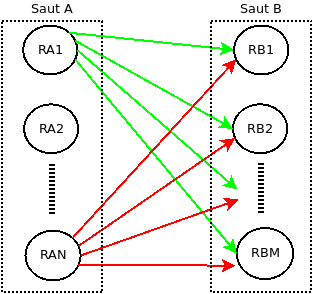
\includegraphics[width=0.5\linewidth]{illustrations/link-inference}
	% Graphic for TeX using PGF
% Title: /home/hayat/RipeAtlasTraceroutesAnalysis/report/illustrations/link-inference.dia
% Creator: Dia v0.97+git
% CreationDate: Thu Nov 29 20:58:09 2018
% For: hayat
% \usepackage{tikz}
% The following commands are not supported in PSTricks at present
% We define them conditionally, so when they are implemented,
% this pgf file will use them.
\ifx\du\undefined
  \newlength{\du}
\fi
\setlength{\du}{15\unitlength}
\begin{tikzpicture}[even odd rule]
\pgftransformxscale{1.000000}
\pgftransformyscale{-1.000000}
\definecolor{dialinecolor}{rgb}{0.000000, 0.000000, 0.000000}
\pgfsetstrokecolor{dialinecolor}
\pgfsetstrokeopacity{1.000000}
\definecolor{diafillcolor}{rgb}{1.000000, 1.000000, 1.000000}
\pgfsetfillcolor{diafillcolor}
\pgfsetfillopacity{1.000000}
\pgfsetlinewidth{0.100000\du}
\pgfsetdash{}{0pt}
\pgfsetmiterjoin
\definecolor{diafillcolor}{rgb}{1.000000, 1.000000, 1.000000}
\pgfsetfillcolor{diafillcolor}
\pgfsetfillopacity{1.000000}
\pgfpathellipse{\pgfpoint{27.430614\du}{13.298442\du}}{\pgfpoint{1.349214\du}{0\du}}{\pgfpoint{0\du}{1.217042\du}}
\pgfusepath{fill}
\definecolor{dialinecolor}{rgb}{0.000000, 0.000000, 0.000000}
\pgfsetstrokecolor{dialinecolor}
\pgfsetstrokeopacity{1.000000}
\pgfpathellipse{\pgfpoint{27.430614\du}{13.298442\du}}{\pgfpoint{1.349214\du}{0\du}}{\pgfpoint{0\du}{1.217042\du}}
\pgfusepath{stroke}
% setfont left to latex
\definecolor{dialinecolor}{rgb}{0.000000, 0.000000, 0.000000}
\pgfsetstrokecolor{dialinecolor}
\pgfsetstrokeopacity{1.000000}
\definecolor{diafillcolor}{rgb}{0.000000, 0.000000, 0.000000}
\pgfsetfillcolor{diafillcolor}
\pgfsetfillopacity{1.000000}
\node[anchor=base,inner sep=0pt, outer sep=0pt,color=dialinecolor] at (27.430614\du,13.493442\du){$R_{1,1}$};
\pgfsetlinewidth{0.100000\du}
\pgfsetdash{}{0pt}
\pgfsetmiterjoin
\definecolor{diafillcolor}{rgb}{1.000000, 1.000000, 1.000000}
\pgfsetfillcolor{diafillcolor}
\pgfsetfillopacity{1.000000}
\pgfpathellipse{\pgfpoint{27.475614\du}{17.238442\du}}{\pgfpoint{1.349214\du}{0\du}}{\pgfpoint{0\du}{1.217042\du}}
\pgfusepath{fill}
\definecolor{dialinecolor}{rgb}{0.000000, 0.000000, 0.000000}
\pgfsetstrokecolor{dialinecolor}
\pgfsetstrokeopacity{1.000000}
\pgfpathellipse{\pgfpoint{27.475614\du}{17.238442\du}}{\pgfpoint{1.349214\du}{0\du}}{\pgfpoint{0\du}{1.217042\du}}
\pgfusepath{stroke}
% setfont left to latex
\definecolor{dialinecolor}{rgb}{0.000000, 0.000000, 0.000000}
\pgfsetstrokecolor{dialinecolor}
\pgfsetstrokeopacity{1.000000}
\definecolor{diafillcolor}{rgb}{0.000000, 0.000000, 0.000000}
\pgfsetfillcolor{diafillcolor}
\pgfsetfillopacity{1.000000}
\node[anchor=base,inner sep=0pt, outer sep=0pt,color=dialinecolor] at (27.475614\du,17.433442\du){$R_{1,2}$};
\pgfsetlinewidth{0.100000\du}
\pgfsetdash{}{0pt}
\pgfsetmiterjoin
\definecolor{diafillcolor}{rgb}{1.000000, 1.000000, 1.000000}
\pgfsetfillcolor{diafillcolor}
\pgfsetfillopacity{1.000000}
\pgfpathellipse{\pgfpoint{27.570578\du}{23.578496\du}}{\pgfpoint{1.376878\du}{0\du}}{\pgfpoint{0\du}{1.241996\du}}
\pgfusepath{fill}
\definecolor{dialinecolor}{rgb}{0.000000, 0.000000, 0.000000}
\pgfsetstrokecolor{dialinecolor}
\pgfsetstrokeopacity{1.000000}
\pgfpathellipse{\pgfpoint{27.570578\du}{23.578496\du}}{\pgfpoint{1.376878\du}{0\du}}{\pgfpoint{0\du}{1.241996\du}}
\pgfusepath{stroke}
% setfont left to latex
\definecolor{dialinecolor}{rgb}{0.000000, 0.000000, 0.000000}
\pgfsetstrokecolor{dialinecolor}
\pgfsetstrokeopacity{1.000000}
\definecolor{diafillcolor}{rgb}{0.000000, 0.000000, 0.000000}
\pgfsetfillcolor{diafillcolor}
\pgfsetfillopacity{1.000000}
\node[anchor=base,inner sep=0pt, outer sep=0pt,color=dialinecolor] at (27.570578\du,23.773496\du){$R_{1,N}$};
\pgfsetlinewidth{0.300000\du}
\pgfsetdash{{\pgflinewidth}{0.200000\du}}{0cm}
\pgfsetbuttcap
{
\definecolor{diafillcolor}{rgb}{0.000000, 0.000000, 0.000000}
\pgfsetfillcolor{diafillcolor}
\pgfsetfillopacity{1.000000}
% was here!!!
\definecolor{dialinecolor}{rgb}{0.000000, 0.000000, 0.000000}
\pgfsetstrokecolor{dialinecolor}
\pgfsetstrokeopacity{1.000000}
\draw (27.540000\du,18.980000\du)--(27.540000\du,21.480000\du);
}
\pgfsetlinewidth{0.100000\du}
\pgfsetdash{}{0pt}
\pgfsetmiterjoin
\definecolor{diafillcolor}{rgb}{1.000000, 1.000000, 1.000000}
\pgfsetfillcolor{diafillcolor}
\pgfsetfillopacity{1.000000}
\pgfpathellipse{\pgfpoint{37.980536\du}{13.298484\du}}{\pgfpoint{1.355136\du}{0\du}}{\pgfpoint{0\du}{1.222384\du}}
\pgfusepath{fill}
\definecolor{dialinecolor}{rgb}{0.000000, 0.000000, 0.000000}
\pgfsetstrokecolor{dialinecolor}
\pgfsetstrokeopacity{1.000000}
\pgfpathellipse{\pgfpoint{37.980536\du}{13.298484\du}}{\pgfpoint{1.355136\du}{0\du}}{\pgfpoint{0\du}{1.222384\du}}
\pgfusepath{stroke}
% setfont left to latex
\definecolor{dialinecolor}{rgb}{0.000000, 0.000000, 0.000000}
\pgfsetstrokecolor{dialinecolor}
\pgfsetstrokeopacity{1.000000}
\definecolor{diafillcolor}{rgb}{0.000000, 0.000000, 0.000000}
\pgfsetfillcolor{diafillcolor}
\pgfsetfillopacity{1.000000}
\node[anchor=base,inner sep=0pt, outer sep=0pt,color=dialinecolor] at (37.980536\du,13.493484\du){$R_{2,1}$};
\pgfsetlinewidth{0.100000\du}
\pgfsetdash{}{0pt}
\pgfsetmiterjoin
\definecolor{diafillcolor}{rgb}{1.000000, 1.000000, 1.000000}
\pgfsetfillcolor{diafillcolor}
\pgfsetfillopacity{1.000000}
\pgfpathellipse{\pgfpoint{37.925536\du}{17.238484\du}}{\pgfpoint{1.355136\du}{0\du}}{\pgfpoint{0\du}{1.222384\du}}
\pgfusepath{fill}
\definecolor{dialinecolor}{rgb}{0.000000, 0.000000, 0.000000}
\pgfsetstrokecolor{dialinecolor}
\pgfsetstrokeopacity{1.000000}
\pgfpathellipse{\pgfpoint{37.925536\du}{17.238484\du}}{\pgfpoint{1.355136\du}{0\du}}{\pgfpoint{0\du}{1.222384\du}}
\pgfusepath{stroke}
% setfont left to latex
\definecolor{dialinecolor}{rgb}{0.000000, 0.000000, 0.000000}
\pgfsetstrokecolor{dialinecolor}
\pgfsetstrokeopacity{1.000000}
\definecolor{diafillcolor}{rgb}{0.000000, 0.000000, 0.000000}
\pgfsetfillcolor{diafillcolor}
\pgfsetfillopacity{1.000000}
\node[anchor=base,inner sep=0pt, outer sep=0pt,color=dialinecolor] at (37.925536\du,17.433484\du){$R_{2,2}$};
\pgfsetlinewidth{0.100000\du}
\pgfsetdash{}{0pt}
\pgfsetmiterjoin
\definecolor{diafillcolor}{rgb}{1.000000, 1.000000, 1.000000}
\pgfsetfillcolor{diafillcolor}
\pgfsetfillopacity{1.000000}
\pgfpathellipse{\pgfpoint{38.170599\du}{23.478445\du}}{\pgfpoint{1.411299\du}{0\du}}{\pgfpoint{0\du}{1.273045\du}}
\pgfusepath{fill}
\definecolor{dialinecolor}{rgb}{0.000000, 0.000000, 0.000000}
\pgfsetstrokecolor{dialinecolor}
\pgfsetstrokeopacity{1.000000}
\pgfpathellipse{\pgfpoint{38.170599\du}{23.478445\du}}{\pgfpoint{1.411299\du}{0\du}}{\pgfpoint{0\du}{1.273045\du}}
\pgfusepath{stroke}
% setfont left to latex
\definecolor{dialinecolor}{rgb}{0.000000, 0.000000, 0.000000}
\pgfsetstrokecolor{dialinecolor}
\pgfsetstrokeopacity{1.000000}
\definecolor{diafillcolor}{rgb}{0.000000, 0.000000, 0.000000}
\pgfsetfillcolor{diafillcolor}
\pgfsetfillopacity{1.000000}
\node[anchor=base,inner sep=0pt, outer sep=0pt,color=dialinecolor] at (38.170599\du,23.673445\du){$R_{1,M}$};
\pgfsetlinewidth{0.300000\du}
\pgfsetdash{{\pgflinewidth}{0.200000\du}}{0cm}
\pgfsetbuttcap
{
\definecolor{diafillcolor}{rgb}{0.000000, 0.000000, 0.000000}
\pgfsetfillcolor{diafillcolor}
\pgfsetfillopacity{1.000000}
% was here!!!
\definecolor{dialinecolor}{rgb}{0.000000, 0.000000, 0.000000}
\pgfsetstrokecolor{dialinecolor}
\pgfsetstrokeopacity{1.000000}
\draw (37.985000\du,18.970000\du)--(37.985000\du,21.470000\du);
}
\pgfsetlinewidth{0.050000\du}
\pgfsetdash{}{0pt}
\pgfsetbuttcap
{
\definecolor{diafillcolor}{rgb}{0.000000, 1.000000, 0.000000}
\pgfsetfillcolor{diafillcolor}
\pgfsetfillopacity{1.000000}
% was here!!!
\pgfsetarrowsstart{stealth}
\definecolor{dialinecolor}{rgb}{0.000000, 1.000000, 0.000000}
\pgfsetstrokecolor{dialinecolor}
\pgfsetstrokeopacity{1.000000}
\draw (28.384600\du,12.437900\du)--(37.022310\du,12.434128\du);
}
\pgfsetlinewidth{0.050000\du}
\pgfsetdash{}{0pt}
\pgfsetbuttcap
{
\definecolor{diafillcolor}{rgb}{1.000000, 0.000000, 0.000000}
\pgfsetfillcolor{diafillcolor}
\pgfsetfillopacity{1.000000}
% was here!!!
\pgfsetarrowsstart{stealth}
\definecolor{dialinecolor}{rgb}{1.000000, 0.000000, 0.000000}
\pgfsetstrokecolor{dialinecolor}
\pgfsetstrokeopacity{1.000000}
\draw (28.842600\du,24.053700\du)--(37.630518\du,24.654584\du);
}
\pgfsetlinewidth{0.100000\du}
\pgfsetdash{{\pgflinewidth}{0.200000\du}}{0cm}
\pgfsetmiterjoin
\pgfsetbuttcap
{\pgfsetcornersarced{\pgfpoint{0.000000\du}{0.000000\du}}\definecolor{dialinecolor}{rgb}{0.000000, 0.000000, 0.000000}
\pgfsetstrokecolor{dialinecolor}
\pgfsetstrokeopacity{1.000000}
\draw (25.638764\du,11.830038\du)--(25.638764\du,25.156536\du)--(29.721269\du,25.156536\du)--(29.721269\du,11.830038\du)--cycle;
}\pgfsetlinewidth{0.100000\du}
\pgfsetdash{{\pgflinewidth}{0.200000\du}}{0cm}
\pgfsetmiterjoin
\pgfsetbuttcap
{\pgfsetcornersarced{\pgfpoint{0.000000\du}{0.000000\du}}\definecolor{dialinecolor}{rgb}{0.000000, 0.000000, 0.000000}
\pgfsetstrokecolor{dialinecolor}
\pgfsetstrokeopacity{1.000000}
\draw (36.096688\du,11.857262\du)--(36.096688\du,25.128574\du)--(39.871607\du,25.128574\du)--(39.871607\du,11.857262\du)--cycle;
}% setfont left to latex
\definecolor{dialinecolor}{rgb}{0.000000, 0.000000, 0.000000}
\pgfsetstrokecolor{dialinecolor}
\pgfsetstrokeopacity{1.000000}
\definecolor{diafillcolor}{rgb}{0.000000, 0.000000, 0.000000}
\pgfsetfillcolor{diafillcolor}
\pgfsetfillopacity{1.000000}
\node[anchor=base west,inner sep=0pt,outer sep=0pt,color=dialinecolor] at (26.470600\du,11.464400\du){$ h_1 $};
% setfont left to latex
\definecolor{dialinecolor}{rgb}{0.000000, 0.000000, 0.000000}
\pgfsetstrokecolor{dialinecolor}
\pgfsetstrokeopacity{1.000000}
\definecolor{diafillcolor}{rgb}{0.000000, 0.000000, 0.000000}
\pgfsetfillcolor{diafillcolor}
\pgfsetfillopacity{1.000000}
\node[anchor=base west,inner sep=0pt,outer sep=0pt,color=dialinecolor] at (36.898700\du,11.464100\du){$ h_2 $};
\pgfsetlinewidth{0.050000\du}
\pgfsetdash{}{0pt}
\pgfsetbuttcap
{
\definecolor{diafillcolor}{rgb}{0.000000, 0.000000, 1.000000}
\pgfsetfillcolor{diafillcolor}
\pgfsetfillopacity{1.000000}
% was here!!!
\pgfsetarrowsstart{stealth}
\definecolor{dialinecolor}{rgb}{0.000000, 0.000000, 1.000000}
\pgfsetstrokecolor{dialinecolor}
\pgfsetstrokeopacity{1.000000}
\draw (28.779828\du,13.298442\du)--(37.406948\du,16.109148\du);
}
\pgfsetlinewidth{0.050000\du}
\pgfsetdash{}{0pt}
\pgfsetbuttcap
{
\definecolor{diafillcolor}{rgb}{0.000000, 1.000000, 0.000000}
\pgfsetfillcolor{diafillcolor}
\pgfsetfillopacity{1.000000}
% was here!!!
\pgfsetarrowsstart{stealth}
\definecolor{dialinecolor}{rgb}{0.000000, 1.000000, 0.000000}
\pgfsetstrokecolor{dialinecolor}
\pgfsetstrokeopacity{1.000000}
\draw (28.722125\du,16.772700\du)--(36.728554\du,12.830698\du);
}
\pgfsetlinewidth{0.050000\du}
\pgfsetdash{}{0pt}
\pgfsetbuttcap
{
\definecolor{diafillcolor}{rgb}{0.000000, 1.000000, 0.000000}
\pgfsetfillcolor{diafillcolor}
\pgfsetfillopacity{1.000000}
% was here!!!
\pgfsetarrowsstart{stealth}
\definecolor{dialinecolor}{rgb}{0.000000, 1.000000, 0.000000}
\pgfsetstrokecolor{dialinecolor}
\pgfsetstrokeopacity{1.000000}
\draw (28.602774\du,20.095348\du)--(36.625400\du,13.298484\du);
}
\pgfsetlinewidth{0.050000\du}
\pgfsetdash{}{0pt}
\pgfsetbuttcap
{
\definecolor{diafillcolor}{rgb}{0.000000, 1.000000, 0.000000}
\pgfsetfillcolor{diafillcolor}
\pgfsetfillopacity{1.000000}
% was here!!!
\pgfsetarrowsstart{stealth}
\definecolor{dialinecolor}{rgb}{0.000000, 1.000000, 0.000000}
\pgfsetstrokecolor{dialinecolor}
\pgfsetstrokeopacity{1.000000}
\draw (28.097487\du,22.431041\du)--(36.728554\du,13.766270\du);
}
\pgfsetlinewidth{0.050000\du}
\pgfsetdash{}{0pt}
\pgfsetbuttcap
{
\definecolor{diafillcolor}{rgb}{0.000000, 0.000000, 1.000000}
\pgfsetfillcolor{diafillcolor}
\pgfsetfillopacity{1.000000}
% was here!!!
\pgfsetarrowsstart{stealth}
\definecolor{dialinecolor}{rgb}{0.000000, 0.000000, 1.000000}
\pgfsetstrokecolor{dialinecolor}
\pgfsetstrokeopacity{1.000000}
\draw (28.824828\du,17.238442\du)--(36.967310\du,16.374128\du);
}
\pgfsetlinewidth{0.050000\du}
\pgfsetdash{}{0pt}
\pgfsetbuttcap
{
\definecolor{diafillcolor}{rgb}{0.000000, 0.000000, 1.000000}
\pgfsetfillcolor{diafillcolor}
\pgfsetfillopacity{1.000000}
% was here!!!
\pgfsetarrowsstart{stealth}
\definecolor{dialinecolor}{rgb}{0.000000, 0.000000, 1.000000}
\pgfsetstrokecolor{dialinecolor}
\pgfsetstrokeopacity{1.000000}
\draw (28.798511\du,20.486821\du)--(36.673554\du,16.770698\du);
}
\pgfsetlinewidth{0.050000\du}
\pgfsetdash{}{0pt}
\pgfsetbuttcap
{
\definecolor{diafillcolor}{rgb}{0.000000, 0.000000, 1.000000}
\pgfsetfillcolor{diafillcolor}
\pgfsetfillopacity{1.000000}
% was here!!!
\pgfsetarrowsstart{stealth}
\definecolor{dialinecolor}{rgb}{0.000000, 0.000000, 1.000000}
\pgfsetstrokecolor{dialinecolor}
\pgfsetstrokeopacity{1.000000}
\draw (28.544178\du,22.700272\du)--(36.516123\du,17.355037\du);
}
\pgfsetlinewidth{0.050000\du}
\pgfsetdash{}{0pt}
\pgfsetbuttcap
{
\definecolor{diafillcolor}{rgb}{1.000000, 0.000000, 0.000000}
\pgfsetfillcolor{diafillcolor}
\pgfsetfillopacity{1.000000}
% was here!!!
\pgfsetarrowsstart{stealth}
\definecolor{dialinecolor}{rgb}{1.000000, 0.000000, 0.000000}
\pgfsetstrokecolor{dialinecolor}
\pgfsetstrokeopacity{1.000000}
\draw (28.938323\du,20.850332\du)--(36.866729\du,23.965618\du);
}
\pgfsetlinewidth{0.050000\du}
\pgfsetdash{}{0pt}
\pgfsetbuttcap
{
\definecolor{diafillcolor}{rgb}{1.000000, 0.000000, 0.000000}
\pgfsetfillcolor{diafillcolor}
\pgfsetfillopacity{1.000000}
% was here!!!
\pgfsetarrowsstart{stealth}
\definecolor{dialinecolor}{rgb}{1.000000, 0.000000, 0.000000}
\pgfsetstrokecolor{dialinecolor}
\pgfsetstrokeopacity{1.000000}
\draw (28.722125\du,17.704183\du)--(36.712688\du,23.381227\du);
}
\pgfsetlinewidth{0.050000\du}
\pgfsetdash{}{0pt}
\pgfsetbuttcap
{
\definecolor{diafillcolor}{rgb}{1.000000, 0.000000, 0.000000}
\pgfsetfillcolor{diafillcolor}
\pgfsetfillopacity{1.000000}
% was here!!!
\pgfsetarrowsstart{stealth}
\definecolor{dialinecolor}{rgb}{1.000000, 0.000000, 0.000000}
\pgfsetstrokecolor{dialinecolor}
\pgfsetstrokeopacity{1.000000}
\draw (28.677125\du,13.764183\du)--(36.866729\du,22.991272\du);
}
\end{tikzpicture}

	\caption{Inférence des liens possibles entre les routeurs des deux sauts consécutifs RAi et RBj}
	\label{fig:link-inference}
\end{figure}
\paragraph{5. Caractérisation des liens} avec leurs RTTs différentiels. A cette étape, on calcule le RTT différentiel d'un lien, au sein d'un traceroute donné, en calculant la différence entre les RTTs des deux routeurs du lien en question. En plus du RTT différentiel, on note aussi la sonde Atlas ayant effectué la requête traceroute où le lien a été identifié. 

\paragraph{6. Fusion des informations d'un lien} Etant donné qu'un lien (IP1, IP2) peut être identifié plusieurs fois pendant une même période $d_i$ d'une part, et le lien (IP2, IP1) est similaire\footnote{La similarité est mesurée par le RTT différentiel.} au lien  (IP1, IP2) d'autre part, la fusion permet de construire une nouvelle distribution des RTTs différentiels caractérisant le lien (IP1, IP2) qui reprend les RTTs différentiels du lien(IP1, IP2) ainsi que ceux du lien (IP2, IP1).


A la fin de l'étape 6, tous les traceroutes sont préparés. A présent, l'objectif est d'identifier les dates pendant lesquelles des anomalies ont été détectées. Pour ce faire, l'idée du travail de référence est de conserver, pour un lien donné, une référence du RTT différentiel médian.  Cette référence est d'abord comparée avec la médiane courante du RTT différentiel,  puis,  mise à jour,   tout au long de la période d'analyse.

  
  \paragraph{7. Calcul de la médiane des RTTs différentiels et   l'intervalle de confiance courant} du lien analysé. Pour un lien donné, on calcule la médiane des RTTs différentiels d'une $d_i$, ensuite on calcule les deux bornes de l'intervalle de confiance pour $d_i$.
  
 
  
  
  \paragraph{8. Mise à jour de la médiane et de l'intervalle de  référence du lien analysé.} La médiane des RTTs différentiels de référence sont d'abords comparés avec ceux de la période $d_i$ courante. Ensuite, ces références sont mises à jour pour prendre en compte ces nouvelles valeurs. A l'issue de cette comparaison, la liste des dates des anomalies est mise à jour.
  

 \paragraph{9. Comparaison des intervalles de confiance} 

La comparaison de l'état courant du lien avec celui de référence est effectuée en analysant le chevauchement d'intervalles de confiance  courant et de référence. Le délai d'un lien est jugé anormal si son intervalle de confiance courant est inclus dans l'intervalle de confiance de référence. C'est le cas 1 dans la Figure 	\ref{fig:intervals-comparaison},  \textit{referenceLow} et \textit{referenceHight} sont les bornes de l'intervalle de confiance de référence.  \textit{currentLow} et \textit{currentHight} sont les bornes de l'intervalle de confiance courant.

D'après le travail de référence, on distingue quatre cas possibles  illustrés dans la Figure 	\ref{fig:intervals-comparaison}:

\textbf{Cas 1 :} le délai du lien est normal.

\textbf{Cas 2 :} le délai du lien est anormal.

\textbf{Cas 3 :} le délai du lien est anormal.

\textbf{Cas 4 :} le délai du lien est anormal.

Dans le cas où le délai est jugé anormal, on introduit ce qu'on appelle la \textit{déviation}. Cette métrique caractérise l'anomalie détectée. Elle est calculée différemment dans le cas où le délai est anormal.

\begin{figure}[h]
	\centering
	\captionsetup{justification=centering}
	\resizebox{\textwidth}{!}{
		% Graphic for TeX using PGF
% Title: /home/hayat/RipeAtlasTraceroutesAnalysis/report/illustrations/intervals-comparaison.dia
% Creator: Dia v0.97+git
% CreationDate: Tue Dec  4 13:30:20 2018
% For: hayat
% \usepackage{tikz}
% The following commands are not supported in PSTricks at present
% We define them conditionally, so when they are implemented,
% this pgf file will use them.
\ifx\du\undefined
  \newlength{\du}
\fi
\setlength{\du}{15\unitlength}
\begin{tikzpicture}[even odd rule]
\pgftransformxscale{1.000000}
\pgftransformyscale{-1.000000}
\definecolor{dialinecolor}{rgb}{0.000000, 0.000000, 0.000000}
\pgfsetstrokecolor{dialinecolor}
\pgfsetstrokeopacity{1.000000}
\definecolor{diafillcolor}{rgb}{1.000000, 1.000000, 1.000000}
\pgfsetfillcolor{diafillcolor}
\pgfsetfillopacity{1.000000}
\pgfsetlinewidth{0.100000\du}
\pgfsetdash{}{0pt}
\pgfsetbuttcap
{
\definecolor{diafillcolor}{rgb}{0.662745, 0.709804, 0.674510}
\pgfsetfillcolor{diafillcolor}
\pgfsetfillopacity{1.000000}
% was here!!!
}
\definecolor{dialinecolor}{rgb}{0.662745, 0.709804, 0.674510}
\pgfsetstrokecolor{dialinecolor}
\pgfsetstrokeopacity{1.000000}
\draw (14.150000\du,0.400000\du)--(27.000000\du,0.400000\du);
\pgfsetlinewidth{0.100000\du}
\pgfsetdash{}{0pt}
\pgfsetmiterjoin
\pgfsetbuttcap
\definecolor{diafillcolor}{rgb}{0.662745, 0.709804, 0.674510}
\pgfsetfillcolor{diafillcolor}
\pgfsetfillopacity{1.000000}
\fill (13.900000\du,0.550000\du)--(13.900000\du,0.250000\du)--(14.200000\du,0.250000\du)--(14.200000\du,0.550000\du)--cycle;
\definecolor{dialinecolor}{rgb}{0.662745, 0.709804, 0.674510}
\pgfsetstrokecolor{dialinecolor}
\pgfsetstrokeopacity{1.000000}
\draw (14.050000\du,0.700000\du)--(14.050000\du,0.100000\du);
\pgfsetlinewidth{0.100000\du}
\pgfsetdash{}{0pt}
\pgfsetmiterjoin
\pgfsetbuttcap
\definecolor{diafillcolor}{rgb}{0.662745, 0.709804, 0.674510}
\pgfsetfillcolor{diafillcolor}
\pgfsetfillopacity{1.000000}
\fill (27.250000\du,0.250000\du)--(27.250000\du,0.550000\du)--(26.950000\du,0.550000\du)--(26.950000\du,0.250000\du)--cycle;
\definecolor{dialinecolor}{rgb}{0.662745, 0.709804, 0.674510}
\pgfsetstrokecolor{dialinecolor}
\pgfsetstrokeopacity{1.000000}
\draw (27.100000\du,0.100000\du)--(27.100000\du,0.700000\du);
\pgfsetlinewidth{0.100000\du}
\pgfsetdash{}{0pt}
\pgfsetbuttcap
{
\definecolor{diafillcolor}{rgb}{0.000000, 0.000000, 0.000000}
\pgfsetfillcolor{diafillcolor}
\pgfsetfillopacity{1.000000}
% was here!!!
}
\definecolor{dialinecolor}{rgb}{0.000000, 0.000000, 0.000000}
\pgfsetstrokecolor{dialinecolor}
\pgfsetstrokeopacity{1.000000}
\draw (16.150000\du,2.450000\du)--(24.800000\du,2.450000\du);
\pgfsetlinewidth{0.100000\du}
\pgfsetdash{}{0pt}
\pgfsetmiterjoin
\pgfsetbuttcap
\definecolor{diafillcolor}{rgb}{0.000000, 0.000000, 0.000000}
\pgfsetfillcolor{diafillcolor}
\pgfsetfillopacity{1.000000}
\fill (15.900000\du,2.600000\du)--(15.900000\du,2.300000\du)--(16.200000\du,2.300000\du)--(16.200000\du,2.600000\du)--cycle;
\definecolor{dialinecolor}{rgb}{0.000000, 0.000000, 0.000000}
\pgfsetstrokecolor{dialinecolor}
\pgfsetstrokeopacity{1.000000}
\draw (16.050000\du,2.750000\du)--(16.050000\du,2.150000\du);
\pgfsetlinewidth{0.100000\du}
\pgfsetdash{}{0pt}
\pgfsetmiterjoin
\pgfsetbuttcap
\definecolor{diafillcolor}{rgb}{0.000000, 0.000000, 0.000000}
\pgfsetfillcolor{diafillcolor}
\pgfsetfillopacity{1.000000}
\fill (25.050000\du,2.300000\du)--(25.050000\du,2.600000\du)--(24.750000\du,2.600000\du)--(24.750000\du,2.300000\du)--cycle;
\definecolor{dialinecolor}{rgb}{0.000000, 0.000000, 0.000000}
\pgfsetstrokecolor{dialinecolor}
\pgfsetstrokeopacity{1.000000}
\draw (24.900000\du,2.150000\du)--(24.900000\du,2.750000\du);
\pgfsetlinewidth{0.100000\du}
\pgfsetdash{}{0pt}
\pgfsetbuttcap
{
\definecolor{diafillcolor}{rgb}{0.662745, 0.709804, 0.674510}
\pgfsetfillcolor{diafillcolor}
\pgfsetfillopacity{1.000000}
% was here!!!
}
\definecolor{dialinecolor}{rgb}{0.662745, 0.709804, 0.674510}
\pgfsetstrokecolor{dialinecolor}
\pgfsetstrokeopacity{1.000000}
\draw (14.008246\du,11.548114\du)--(26.858246\du,11.548114\du);
\pgfsetlinewidth{0.100000\du}
\pgfsetdash{}{0pt}
\pgfsetmiterjoin
\pgfsetbuttcap
\definecolor{diafillcolor}{rgb}{0.662745, 0.709804, 0.674510}
\pgfsetfillcolor{diafillcolor}
\pgfsetfillopacity{1.000000}
\fill (13.758246\du,11.698114\du)--(13.758246\du,11.398114\du)--(14.058246\du,11.398114\du)--(14.058246\du,11.698114\du)--cycle;
\definecolor{dialinecolor}{rgb}{0.662745, 0.709804, 0.674510}
\pgfsetstrokecolor{dialinecolor}
\pgfsetstrokeopacity{1.000000}
\draw (13.908246\du,11.848114\du)--(13.908246\du,11.248114\du);
\pgfsetlinewidth{0.100000\du}
\pgfsetdash{}{0pt}
\pgfsetmiterjoin
\pgfsetbuttcap
\definecolor{diafillcolor}{rgb}{0.662745, 0.709804, 0.674510}
\pgfsetfillcolor{diafillcolor}
\pgfsetfillopacity{1.000000}
\fill (27.108246\du,11.398114\du)--(27.108246\du,11.698114\du)--(26.808246\du,11.698114\du)--(26.808246\du,11.398114\du)--cycle;
\definecolor{dialinecolor}{rgb}{0.662745, 0.709804, 0.674510}
\pgfsetstrokecolor{dialinecolor}
\pgfsetstrokeopacity{1.000000}
\draw (26.958246\du,11.248114\du)--(26.958246\du,11.848114\du);
\pgfsetlinewidth{0.100000\du}
\pgfsetdash{}{0pt}
\pgfsetbuttcap
{
\definecolor{diafillcolor}{rgb}{0.000000, 0.000000, 0.000000}
\pgfsetfillcolor{diafillcolor}
\pgfsetfillopacity{1.000000}
% was here!!!
}
\definecolor{dialinecolor}{rgb}{0.000000, 0.000000, 0.000000}
\pgfsetstrokecolor{dialinecolor}
\pgfsetstrokeopacity{1.000000}
\draw (23.108246\du,13.598114\du)--(31.758246\du,13.598114\du);
\pgfsetlinewidth{0.100000\du}
\pgfsetdash{}{0pt}
\pgfsetmiterjoin
\pgfsetbuttcap
\definecolor{diafillcolor}{rgb}{0.000000, 0.000000, 0.000000}
\pgfsetfillcolor{diafillcolor}
\pgfsetfillopacity{1.000000}
\fill (22.858246\du,13.748114\du)--(22.858246\du,13.448114\du)--(23.158246\du,13.448114\du)--(23.158246\du,13.748114\du)--cycle;
\definecolor{dialinecolor}{rgb}{0.000000, 0.000000, 0.000000}
\pgfsetstrokecolor{dialinecolor}
\pgfsetstrokeopacity{1.000000}
\draw (23.008246\du,13.898114\du)--(23.008246\du,13.298114\du);
\pgfsetlinewidth{0.100000\du}
\pgfsetdash{}{0pt}
\pgfsetmiterjoin
\pgfsetbuttcap
\definecolor{diafillcolor}{rgb}{0.000000, 0.000000, 0.000000}
\pgfsetfillcolor{diafillcolor}
\pgfsetfillopacity{1.000000}
\fill (32.008246\du,13.448114\du)--(32.008246\du,13.748114\du)--(31.708246\du,13.748114\du)--(31.708246\du,13.448114\du)--cycle;
\definecolor{dialinecolor}{rgb}{0.000000, 0.000000, 0.000000}
\pgfsetstrokecolor{dialinecolor}
\pgfsetstrokeopacity{1.000000}
\draw (31.858246\du,13.298114\du)--(31.858246\du,13.898114\du);
\pgfsetlinewidth{0.100000\du}
\pgfsetdash{}{0pt}
\pgfsetbuttcap
{
\definecolor{diafillcolor}{rgb}{0.662745, 0.709804, 0.674510}
\pgfsetfillcolor{diafillcolor}
\pgfsetfillopacity{1.000000}
% was here!!!
}
\definecolor{dialinecolor}{rgb}{0.662745, 0.709804, 0.674510}
\pgfsetstrokecolor{dialinecolor}
\pgfsetstrokeopacity{1.000000}
\draw (14.108246\du,17.048114\du)--(26.958246\du,17.048114\du);
\pgfsetlinewidth{0.100000\du}
\pgfsetdash{}{0pt}
\pgfsetmiterjoin
\pgfsetbuttcap
\definecolor{diafillcolor}{rgb}{0.662745, 0.709804, 0.674510}
\pgfsetfillcolor{diafillcolor}
\pgfsetfillopacity{1.000000}
\fill (13.858246\du,17.198114\du)--(13.858246\du,16.898114\du)--(14.158246\du,16.898114\du)--(14.158246\du,17.198114\du)--cycle;
\definecolor{dialinecolor}{rgb}{0.662745, 0.709804, 0.674510}
\pgfsetstrokecolor{dialinecolor}
\pgfsetstrokeopacity{1.000000}
\draw (14.008246\du,17.348114\du)--(14.008246\du,16.748114\du);
\pgfsetlinewidth{0.100000\du}
\pgfsetdash{}{0pt}
\pgfsetmiterjoin
\pgfsetbuttcap
\definecolor{diafillcolor}{rgb}{0.662745, 0.709804, 0.674510}
\pgfsetfillcolor{diafillcolor}
\pgfsetfillopacity{1.000000}
\fill (27.208246\du,16.898114\du)--(27.208246\du,17.198114\du)--(26.908246\du,17.198114\du)--(26.908246\du,16.898114\du)--cycle;
\definecolor{dialinecolor}{rgb}{0.662745, 0.709804, 0.674510}
\pgfsetstrokecolor{dialinecolor}
\pgfsetstrokeopacity{1.000000}
\draw (27.058246\du,16.748114\du)--(27.058246\du,17.348114\du);
\pgfsetlinewidth{0.100000\du}
\pgfsetdash{}{0pt}
\pgfsetbuttcap
{
\definecolor{diafillcolor}{rgb}{0.000000, 0.000000, 0.000000}
\pgfsetfillcolor{diafillcolor}
\pgfsetfillopacity{1.000000}
% was here!!!
}
\definecolor{dialinecolor}{rgb}{0.000000, 0.000000, 0.000000}
\pgfsetstrokecolor{dialinecolor}
\pgfsetstrokeopacity{1.000000}
\draw (9.308246\du,19.048114\du)--(17.958246\du,19.048114\du);
\pgfsetlinewidth{0.100000\du}
\pgfsetdash{}{0pt}
\pgfsetmiterjoin
\pgfsetbuttcap
\definecolor{diafillcolor}{rgb}{0.000000, 0.000000, 0.000000}
\pgfsetfillcolor{diafillcolor}
\pgfsetfillopacity{1.000000}
\fill (9.058246\du,19.198114\du)--(9.058246\du,18.898114\du)--(9.358246\du,18.898114\du)--(9.358246\du,19.198114\du)--cycle;
\definecolor{dialinecolor}{rgb}{0.000000, 0.000000, 0.000000}
\pgfsetstrokecolor{dialinecolor}
\pgfsetstrokeopacity{1.000000}
\draw (9.208246\du,19.348114\du)--(9.208246\du,18.748114\du);
\pgfsetlinewidth{0.100000\du}
\pgfsetdash{}{0pt}
\pgfsetmiterjoin
\pgfsetbuttcap
\definecolor{diafillcolor}{rgb}{0.000000, 0.000000, 0.000000}
\pgfsetfillcolor{diafillcolor}
\pgfsetfillopacity{1.000000}
\fill (18.208246\du,18.898114\du)--(18.208246\du,19.198114\du)--(17.908246\du,19.198114\du)--(17.908246\du,18.898114\du)--cycle;
\definecolor{dialinecolor}{rgb}{0.000000, 0.000000, 0.000000}
\pgfsetstrokecolor{dialinecolor}
\pgfsetstrokeopacity{1.000000}
\draw (18.058246\du,18.748114\du)--(18.058246\du,19.348114\du);
\pgfsetlinewidth{0.100000\du}
\pgfsetdash{{\pgflinewidth}{0.200000\du}}{0cm}
\pgfsetbuttcap
{
\definecolor{diafillcolor}{rgb}{0.000000, 0.000000, 0.000000}
\pgfsetfillcolor{diafillcolor}
\pgfsetfillopacity{1.000000}
% was here!!!
\pgfsetarrowsend{stealth}
\definecolor{dialinecolor}{rgb}{0.000000, 0.000000, 0.000000}
\pgfsetstrokecolor{dialinecolor}
\pgfsetstrokeopacity{1.000000}
\draw (5.050000\du,21.000000\du)--(38.800000\du,20.950000\du);
}
\pgfsetlinewidth{0.100000\du}
\pgfsetdash{}{0pt}
\pgfsetbuttcap
{
\definecolor{diafillcolor}{rgb}{0.662745, 0.709804, 0.674510}
\pgfsetfillcolor{diafillcolor}
\pgfsetfillopacity{1.000000}
% was here!!!
}
\definecolor{dialinecolor}{rgb}{0.662745, 0.709804, 0.674510}
\pgfsetstrokecolor{dialinecolor}
\pgfsetstrokeopacity{1.000000}
\draw (13.958246\du,6.048114\du)--(26.808246\du,6.048114\du);
\pgfsetlinewidth{0.100000\du}
\pgfsetdash{}{0pt}
\pgfsetmiterjoin
\pgfsetbuttcap
\definecolor{diafillcolor}{rgb}{0.662745, 0.709804, 0.674510}
\pgfsetfillcolor{diafillcolor}
\pgfsetfillopacity{1.000000}
\fill (13.708246\du,6.198114\du)--(13.708246\du,5.898114\du)--(14.008246\du,5.898114\du)--(14.008246\du,6.198114\du)--cycle;
\definecolor{dialinecolor}{rgb}{0.662745, 0.709804, 0.674510}
\pgfsetstrokecolor{dialinecolor}
\pgfsetstrokeopacity{1.000000}
\draw (13.858246\du,6.348114\du)--(13.858246\du,5.748114\du);
\pgfsetlinewidth{0.100000\du}
\pgfsetdash{}{0pt}
\pgfsetmiterjoin
\pgfsetbuttcap
\definecolor{diafillcolor}{rgb}{0.662745, 0.709804, 0.674510}
\pgfsetfillcolor{diafillcolor}
\pgfsetfillopacity{1.000000}
\fill (27.058246\du,5.898114\du)--(27.058246\du,6.198114\du)--(26.758246\du,6.198114\du)--(26.758246\du,5.898114\du)--cycle;
\definecolor{dialinecolor}{rgb}{0.662745, 0.709804, 0.674510}
\pgfsetstrokecolor{dialinecolor}
\pgfsetstrokeopacity{1.000000}
\draw (26.908246\du,5.748114\du)--(26.908246\du,6.348114\du);
\pgfsetlinewidth{0.100000\du}
\pgfsetdash{}{0pt}
\pgfsetbuttcap
{
\definecolor{diafillcolor}{rgb}{0.000000, 0.000000, 0.000000}
\pgfsetfillcolor{diafillcolor}
\pgfsetfillopacity{1.000000}
% was here!!!
}
\definecolor{dialinecolor}{rgb}{0.000000, 0.000000, 0.000000}
\pgfsetstrokecolor{dialinecolor}
\pgfsetstrokeopacity{1.000000}
\draw (10.049999\du,8.049461\du)--(32.750001\du,8.000539\du);
\pgfsetlinewidth{0.100000\du}
\pgfsetdash{}{0pt}
\pgfsetmiterjoin
\pgfsetbuttcap
\definecolor{diafillcolor}{rgb}{0.000000, 0.000000, 0.000000}
\pgfsetfillcolor{diafillcolor}
\pgfsetfillopacity{1.000000}
\fill (9.800323\du,8.200000\du)--(9.799677\du,7.900000\du)--(10.099676\du,7.899354\du)--(10.100323\du,8.199353\du)--cycle;
\definecolor{dialinecolor}{rgb}{0.000000, 0.000000, 0.000000}
\pgfsetstrokecolor{dialinecolor}
\pgfsetstrokeopacity{1.000000}
\draw (9.950646\du,8.349676\du)--(9.949353\du,7.749677\du);
\pgfsetlinewidth{0.100000\du}
\pgfsetdash{}{0pt}
\pgfsetmiterjoin
\pgfsetbuttcap
\definecolor{diafillcolor}{rgb}{0.000000, 0.000000, 0.000000}
\pgfsetfillcolor{diafillcolor}
\pgfsetfillopacity{1.000000}
\fill (32.999677\du,7.850000\du)--(33.000323\du,8.150000\du)--(32.700324\du,8.150646\du)--(32.699677\du,7.850647\du)--cycle;
\definecolor{dialinecolor}{rgb}{0.000000, 0.000000, 0.000000}
\pgfsetstrokecolor{dialinecolor}
\pgfsetstrokeopacity{1.000000}
\draw (32.849354\du,7.700324\du)--(32.850647\du,8.300323\du);
\pgfsetlinewidth{0.050000\du}
\pgfsetdash{}{0pt}
\pgfsetmiterjoin
\pgfsetbuttcap
{\pgfsetcornersarced{\pgfpoint{0.000000\du}{0.000000\du}}\definecolor{dialinecolor}{rgb}{0.000000, 0.000000, 0.000000}
\pgfsetstrokecolor{dialinecolor}
\pgfsetstrokeopacity{1.000000}
\draw (6.900000\du,4.500000\du)--(6.900000\du,8.950000\du)--(36.950000\du,8.950000\du)--(36.950000\du,4.500000\du)--cycle;
}% setfont left to latex
\definecolor{dialinecolor}{rgb}{0.000000, 0.000000, 0.000000}
\pgfsetstrokecolor{dialinecolor}
\pgfsetstrokeopacity{1.000000}
\definecolor{diafillcolor}{rgb}{0.000000, 0.000000, 0.000000}
\pgfsetfillcolor{diafillcolor}
\pgfsetfillopacity{1.000000}
\node[anchor=base west,inner sep=0pt,outer sep=0pt,color=dialinecolor] at (7.950000\du,7.550000\du){currentLow};
% setfont left to latex
\definecolor{dialinecolor}{rgb}{0.000000, 0.000000, 0.000000}
\pgfsetstrokecolor{dialinecolor}
\pgfsetstrokeopacity{1.000000}
\definecolor{diafillcolor}{rgb}{0.000000, 0.000000, 0.000000}
\pgfsetfillcolor{diafillcolor}
\pgfsetfillopacity{1.000000}
\node[anchor=base west,inner sep=0pt,outer sep=0pt,color=dialinecolor] at (30.800000\du,7.500000\du){currentHight};
% setfont left to latex
\definecolor{dialinecolor}{rgb}{0.282353, 0.313726, 0.290196}
\pgfsetstrokecolor{dialinecolor}
\pgfsetstrokeopacity{1.000000}
\definecolor{diafillcolor}{rgb}{0.282353, 0.313726, 0.290196}
\pgfsetfillcolor{diafillcolor}
\pgfsetfillopacity{1.000000}
\node[anchor=base west,inner sep=0pt,outer sep=0pt,color=dialinecolor] at (11.450000\du,5.550000\du){referenceLow};
% setfont left to latex
\definecolor{dialinecolor}{rgb}{0.282353, 0.313726, 0.290196}
\pgfsetstrokecolor{dialinecolor}
\pgfsetstrokeopacity{1.000000}
\definecolor{diafillcolor}{rgb}{0.282353, 0.313726, 0.290196}
\pgfsetfillcolor{diafillcolor}
\pgfsetfillopacity{1.000000}
\node[anchor=base west,inner sep=0pt,outer sep=0pt,color=dialinecolor] at (23.750000\du,5.550000\du){referenceHight};
% setfont left to latex
\definecolor{dialinecolor}{rgb}{0.282353, 0.313726, 0.290196}
\pgfsetstrokecolor{dialinecolor}
\pgfsetstrokeopacity{1.000000}
\definecolor{diafillcolor}{rgb}{0.282353, 0.313726, 0.290196}
\pgfsetfillcolor{diafillcolor}
\pgfsetfillopacity{1.000000}
\node[anchor=base west,inner sep=0pt,outer sep=0pt,color=dialinecolor] at (24.545000\du,-0.297500\du){referenceHight};
% setfont left to latex
\definecolor{dialinecolor}{rgb}{0.282353, 0.313726, 0.290196}
\pgfsetstrokecolor{dialinecolor}
\pgfsetstrokeopacity{1.000000}
\definecolor{diafillcolor}{rgb}{0.282353, 0.313726, 0.290196}
\pgfsetfillcolor{diafillcolor}
\pgfsetfillopacity{1.000000}
\node[anchor=base west,inner sep=0pt,outer sep=0pt,color=dialinecolor] at (24.390000\du,10.792500\du){referenceHight};
% setfont left to latex
\definecolor{dialinecolor}{rgb}{0.282353, 0.313726, 0.290196}
\pgfsetstrokecolor{dialinecolor}
\pgfsetstrokeopacity{1.000000}
\definecolor{diafillcolor}{rgb}{0.282353, 0.313726, 0.290196}
\pgfsetfillcolor{diafillcolor}
\pgfsetfillopacity{1.000000}
\node[anchor=base west,inner sep=0pt,outer sep=0pt,color=dialinecolor] at (24.485000\du,16.282500\du){referenceHight};
% setfont left to latex
\definecolor{dialinecolor}{rgb}{0.282353, 0.313726, 0.290196}
\pgfsetstrokecolor{dialinecolor}
\pgfsetstrokeopacity{1.000000}
\definecolor{diafillcolor}{rgb}{0.282353, 0.313726, 0.290196}
\pgfsetfillcolor{diafillcolor}
\pgfsetfillopacity{1.000000}
\node[anchor=base west,inner sep=0pt,outer sep=0pt,color=dialinecolor] at (12.045000\du,-0.247500\du){referenceLow};
% setfont left to latex
\definecolor{dialinecolor}{rgb}{0.282353, 0.313726, 0.290196}
\pgfsetstrokecolor{dialinecolor}
\pgfsetstrokeopacity{1.000000}
\definecolor{diafillcolor}{rgb}{0.282353, 0.313726, 0.290196}
\pgfsetfillcolor{diafillcolor}
\pgfsetfillopacity{1.000000}
\node[anchor=base west,inner sep=0pt,outer sep=0pt,color=dialinecolor] at (11.340000\du,10.892500\du){referenceLow};
% setfont left to latex
\definecolor{dialinecolor}{rgb}{0.282353, 0.313726, 0.290196}
\pgfsetstrokecolor{dialinecolor}
\pgfsetstrokeopacity{1.000000}
\definecolor{diafillcolor}{rgb}{0.282353, 0.313726, 0.290196}
\pgfsetfillcolor{diafillcolor}
\pgfsetfillopacity{1.000000}
\node[anchor=base west,inner sep=0pt,outer sep=0pt,color=dialinecolor] at (11.535000\du,16.532500\du){referenceLow};
% setfont left to latex
\definecolor{dialinecolor}{rgb}{0.000000, 0.000000, 0.000000}
\pgfsetstrokecolor{dialinecolor}
\pgfsetstrokeopacity{1.000000}
\definecolor{diafillcolor}{rgb}{0.000000, 0.000000, 0.000000}
\pgfsetfillcolor{diafillcolor}
\pgfsetfillopacity{1.000000}
\node[anchor=base west,inner sep=0pt,outer sep=0pt,color=dialinecolor] at (13.845000\du,2.002500\du){currentLow};
% setfont left to latex
\definecolor{dialinecolor}{rgb}{0.000000, 0.000000, 0.000000}
\pgfsetstrokecolor{dialinecolor}
\pgfsetstrokeopacity{1.000000}
\definecolor{diafillcolor}{rgb}{0.000000, 0.000000, 0.000000}
\pgfsetfillcolor{diafillcolor}
\pgfsetfillopacity{1.000000}
\node[anchor=base west,inner sep=0pt,outer sep=0pt,color=dialinecolor] at (22.745000\du,2.002500\du){currentHight};
\pgfsetlinewidth{0.050000\du}
\pgfsetdash{}{0pt}
\pgfsetmiterjoin
\pgfsetbuttcap
{\pgfsetcornersarced{\pgfpoint{0.000000\du}{0.000000\du}}\definecolor{dialinecolor}{rgb}{0.000000, 0.000000, 0.000000}
\pgfsetstrokecolor{dialinecolor}
\pgfsetstrokeopacity{1.000000}
\draw (7.000000\du,-1.085000\du)--(7.000000\du,3.365000\du)--(37.000000\du,3.365000\du)--(37.000000\du,-1.085000\du)--cycle;
}% setfont left to latex
\definecolor{dialinecolor}{rgb}{0.000000, 0.000000, 0.000000}
\pgfsetstrokecolor{dialinecolor}
\pgfsetstrokeopacity{1.000000}
\definecolor{diafillcolor}{rgb}{0.000000, 0.000000, 0.000000}
\pgfsetfillcolor{diafillcolor}
\pgfsetfillopacity{1.000000}
\node[anchor=base west,inner sep=0pt,outer sep=0pt,color=dialinecolor] at (20.895000\du,13.002500\du){currentLow};
% setfont left to latex
\definecolor{dialinecolor}{rgb}{0.000000, 0.000000, 0.000000}
\pgfsetstrokecolor{dialinecolor}
\pgfsetstrokeopacity{1.000000}
\definecolor{diafillcolor}{rgb}{0.000000, 0.000000, 0.000000}
\pgfsetfillcolor{diafillcolor}
\pgfsetfillopacity{1.000000}
\node[anchor=base west,inner sep=0pt,outer sep=0pt,color=dialinecolor] at (7.140000\du,18.292500\du){currentLow};
% setfont left to latex
\definecolor{dialinecolor}{rgb}{0.000000, 0.000000, 0.000000}
\pgfsetstrokecolor{dialinecolor}
\pgfsetstrokeopacity{1.000000}
\definecolor{diafillcolor}{rgb}{0.000000, 0.000000, 0.000000}
\pgfsetfillcolor{diafillcolor}
\pgfsetfillopacity{1.000000}
\node[anchor=base west,inner sep=0pt,outer sep=0pt,color=dialinecolor] at (29.695000\du,13.002500\du){currentHight};
% setfont left to latex
\definecolor{dialinecolor}{rgb}{0.000000, 0.000000, 0.000000}
\pgfsetstrokecolor{dialinecolor}
\pgfsetstrokeopacity{1.000000}
\definecolor{diafillcolor}{rgb}{0.000000, 0.000000, 0.000000}
\pgfsetfillcolor{diafillcolor}
\pgfsetfillopacity{1.000000}
\node[anchor=base west,inner sep=0pt,outer sep=0pt,color=dialinecolor] at (15.840000\du,18.442500\du){currentHight};
\pgfsetlinewidth{0.050000\du}
\pgfsetdash{}{0pt}
\pgfsetmiterjoin
\pgfsetbuttcap
{\pgfsetcornersarced{\pgfpoint{0.000000\du}{0.000000\du}}\definecolor{dialinecolor}{rgb}{0.000000, 0.000000, 0.000000}
\pgfsetstrokecolor{dialinecolor}
\pgfsetstrokeopacity{1.000000}
\draw (7.000000\du,10.015000\du)--(7.000000\du,14.465000\du)--(37.050000\du,14.465000\du)--(37.050000\du,10.015000\du)--cycle;
}\pgfsetlinewidth{0.050000\du}
\pgfsetdash{}{0pt}
\pgfsetmiterjoin
\pgfsetbuttcap
{\pgfsetcornersarced{\pgfpoint{0.000000\du}{0.000000\du}}\definecolor{dialinecolor}{rgb}{0.000000, 0.000000, 0.000000}
\pgfsetstrokecolor{dialinecolor}
\pgfsetstrokeopacity{1.000000}
\draw (6.950000\du,15.515000\du)--(6.950000\du,19.965000\du)--(37.050000\du,19.965000\du)--(37.050000\du,15.515000\du)--cycle;
}% setfont left to latex
\definecolor{dialinecolor}{rgb}{0.000000, 0.000000, 0.000000}
\pgfsetstrokecolor{dialinecolor}
\pgfsetstrokeopacity{1.000000}
\definecolor{diafillcolor}{rgb}{0.000000, 0.000000, 0.000000}
\pgfsetfillcolor{diafillcolor}
\pgfsetfillopacity{1.000000}
\node[anchor=base west,inner sep=0pt,outer sep=0pt,color=dialinecolor] at (3.950000\du,1.000000\du){Cas 1};
% setfont left to latex
\definecolor{dialinecolor}{rgb}{0.000000, 0.000000, 0.000000}
\pgfsetstrokecolor{dialinecolor}
\pgfsetstrokeopacity{1.000000}
\definecolor{diafillcolor}{rgb}{0.000000, 0.000000, 0.000000}
\pgfsetfillcolor{diafillcolor}
\pgfsetfillopacity{1.000000}
\node[anchor=base west,inner sep=0pt,outer sep=0pt,color=dialinecolor] at (4.050000\du,7.000000\du){Cas 2};
% setfont left to latex
\definecolor{dialinecolor}{rgb}{0.000000, 0.000000, 0.000000}
\pgfsetstrokecolor{dialinecolor}
\pgfsetstrokeopacity{1.000000}
\definecolor{diafillcolor}{rgb}{0.000000, 0.000000, 0.000000}
\pgfsetfillcolor{diafillcolor}
\pgfsetfillopacity{1.000000}
\node[anchor=base west,inner sep=0pt,outer sep=0pt,color=dialinecolor] at (4.050000\du,12.000000\du){Cas 3};
% setfont left to latex
\definecolor{dialinecolor}{rgb}{0.000000, 0.000000, 0.000000}
\pgfsetstrokecolor{dialinecolor}
\pgfsetstrokeopacity{1.000000}
\definecolor{diafillcolor}{rgb}{0.000000, 0.000000, 0.000000}
\pgfsetfillcolor{diafillcolor}
\pgfsetfillopacity{1.000000}
\node[anchor=base west,inner sep=0pt,outer sep=0pt,color=dialinecolor] at (4.050000\du,18.100000\du){Cas 4};
\end{tikzpicture}

	}
	\caption{La comparaison des deux intervalles de confiance : courant et référence }
	\label{fig:intervals-comparaison}
\end{figure}

\subsection{Vue globale des étapes de la détection des anomalies à travers l'évolution des RTTs différentiels}
La figure 	\ref{fig:process-rttanalysis_tex} présente la succession des étapes de la détection des anomalies dans les délais d'un lien donné. 

\begin{figure}[h]
	\centering
	\resizebox{\textwidth}{\textheight}{
		% Graphic for TeX using PGF
% Title: /home/hayat/RipeAtlasTraceroutesAnalysis/dia/process-rttanalysis.dia
% Creator: Dia v0.97+git
% CreationDate: Thu Nov 29 01:56:23 2018
% For: hayat
% \usepackage{tikz}
% The following commands are not supported in PSTricks at present
% We define them conditionally, so when they are implemented,
% this pgf file will use them.
\ifx\du\undefined
  \newlength{\du}
\fi
\setlength{\du}{15\unitlength}
\begin{tikzpicture}[even odd rule]
\pgftransformxscale{1.000000}
\pgftransformyscale{-1.000000}
\definecolor{dialinecolor}{rgb}{0.000000, 0.000000, 0.000000}
\pgfsetstrokecolor{dialinecolor}
\pgfsetstrokeopacity{1.000000}
\definecolor{diafillcolor}{rgb}{1.000000, 1.000000, 1.000000}
\pgfsetfillcolor{diafillcolor}
\pgfsetfillopacity{1.000000}
\pgfsetlinewidth{0.100000\du}
\pgfsetdash{}{0pt}
\pgfsetmiterjoin
{\pgfsetcornersarced{\pgfpoint{0.000000\du}{0.000000\du}}\definecolor{diafillcolor}{rgb}{1.000000, 1.000000, 1.000000}
\pgfsetfillcolor{diafillcolor}
\pgfsetfillopacity{1.000000}
\fill (8.138750\du,-5.900000\du)--(8.138750\du,-4.000000\du)--(21.861250\du,-4.000000\du)--(21.861250\du,-5.900000\du)--cycle;
}{\pgfsetcornersarced{\pgfpoint{0.000000\du}{0.000000\du}}\definecolor{dialinecolor}{rgb}{0.000000, 0.000000, 0.000000}
\pgfsetstrokecolor{dialinecolor}
\pgfsetstrokeopacity{1.000000}
\draw (8.138750\du,-5.900000\du)--(8.138750\du,-4.000000\du)--(21.861250\du,-4.000000\du)--(21.861250\du,-5.900000\du)--cycle;
}% setfont left to latex
\definecolor{dialinecolor}{rgb}{0.000000, 0.000000, 0.000000}
\pgfsetstrokecolor{dialinecolor}
\pgfsetstrokeopacity{1.000000}
\definecolor{diafillcolor}{rgb}{0.000000, 0.000000, 0.000000}
\pgfsetfillcolor{diafillcolor}
\pgfsetfillopacity{1.000000}
\node[anchor=base,inner sep=0pt, outer sep=0pt,color=dialinecolor] at (15.000000\du,-4.755000\du){\ensuremath{[}traceroute:\{from:"",type:"", result:""\}\ensuremath{]}};
\pgfsetlinewidth{0.100000\du}
\pgfsetdash{}{0pt}
\pgfsetbuttcap
{
\definecolor{diafillcolor}{rgb}{0.000000, 0.000000, 0.000000}
\pgfsetfillcolor{diafillcolor}
\pgfsetfillopacity{1.000000}
% was here!!!
\pgfsetarrowsend{stealth}
\definecolor{dialinecolor}{rgb}{0.000000, 0.000000, 0.000000}
\pgfsetstrokecolor{dialinecolor}
\pgfsetstrokeopacity{1.000000}
\draw (20.060900\du,1.256430\du)--(15.048400\du,4.142720\du);
}
\pgfsetlinewidth{0.100000\du}
\pgfsetdash{}{0pt}
\pgfsetmiterjoin
{\pgfsetcornersarced{\pgfpoint{0.000000\du}{0.000000\du}}\definecolor{diafillcolor}{rgb}{1.000000, 1.000000, 1.000000}
\pgfsetfillcolor{diafillcolor}
\pgfsetfillopacity{1.000000}
\fill (4.175940\du,4.142080\du)--(4.175940\du,6.042080\du)--(9.163440\du,6.042080\du)--(9.163440\du,4.142080\du)--cycle;
}{\pgfsetcornersarced{\pgfpoint{0.000000\du}{0.000000\du}}\definecolor{dialinecolor}{rgb}{0.000000, 0.000000, 0.000000}
\pgfsetstrokecolor{dialinecolor}
\pgfsetstrokeopacity{1.000000}
\draw (4.175940\du,4.142080\du)--(4.175940\du,6.042080\du)--(9.163440\du,6.042080\du)--(9.163440\du,4.142080\du)--cycle;
}% setfont left to latex
\definecolor{dialinecolor}{rgb}{0.000000, 0.000000, 0.000000}
\pgfsetstrokecolor{dialinecolor}
\pgfsetstrokeopacity{1.000000}
\definecolor{diafillcolor}{rgb}{0.000000, 0.000000, 0.000000}
\pgfsetfillcolor{diafillcolor}
\pgfsetfillopacity{1.000000}
\node[anchor=base,inner sep=0pt, outer sep=0pt,color=dialinecolor] at (6.669690\du,5.287080\du){\ensuremath{[}Traceroute\ensuremath{]}};
% setfont left to latex
\definecolor{dialinecolor}{rgb}{0.000000, 0.000000, 0.000000}
\pgfsetstrokecolor{dialinecolor}
\pgfsetstrokeopacity{1.000000}
\definecolor{diafillcolor}{rgb}{0.000000, 0.000000, 0.000000}
\pgfsetfillcolor{diafillcolor}
\pgfsetfillopacity{1.000000}
\node[anchor=base west,inner sep=0pt,outer sep=0pt,color=dialinecolor] at (16.400000\du,9.562040\du){};
\pgfsetlinewidth{0.100000\du}
\pgfsetdash{}{0pt}
\pgfsetbuttcap
\pgfsetmiterjoin
\pgfsetlinewidth{0.100000\du}
\pgfsetbuttcap
\pgfsetmiterjoin
\pgfsetdash{}{0pt}
\definecolor{diafillcolor}{rgb}{1.000000, 1.000000, 1.000000}
\pgfsetfillcolor{diafillcolor}
\pgfsetfillopacity{1.000000}
\definecolor{dialinecolor}{rgb}{0.000000, 0.000000, 0.000000}
\pgfsetstrokecolor{dialinecolor}
\pgfsetstrokeopacity{1.000000}
\pgfpathmoveto{\pgfpoint{24.362725\du}{6.967570\du}}
\pgfpathlineto{\pgfpoint{38.555225\du}{6.967570\du}}
\pgfpathcurveto{\pgfpoint{40.514801\du}{6.967570\du}}{\pgfpoint{42.103350\du}{7.213813\du}}{\pgfpoint{42.103350\du}{7.517570\du}}
\pgfpathcurveto{\pgfpoint{42.103350\du}{7.821327\du}}{\pgfpoint{40.514801\du}{8.067570\du}}{\pgfpoint{38.555225\du}{8.067570\du}}
\pgfpathlineto{\pgfpoint{24.362725\du}{8.067570\du}}
\pgfpathcurveto{\pgfpoint{22.403149\du}{8.067570\du}}{\pgfpoint{20.814600\du}{7.821327\du}}{\pgfpoint{20.814600\du}{7.517570\du}}
\pgfpathcurveto{\pgfpoint{20.814600\du}{7.213813\du}}{\pgfpoint{22.403149\du}{6.967570\du}}{\pgfpoint{24.362725\du}{6.967570\du}}
\pgfpathclose
\pgfusepath{fill,stroke}
% setfont left to latex
\definecolor{dialinecolor}{rgb}{0.000000, 0.000000, 0.000000}
\pgfsetstrokecolor{dialinecolor}
\pgfsetstrokeopacity{1.000000}
\definecolor{diafillcolor}{rgb}{0.000000, 0.000000, 0.000000}
\pgfsetfillcolor{diafillcolor}
\pgfsetfillopacity{1.000000}
\node[anchor=base,inner sep=0pt, outer sep=0pt,color=dialinecolor] at (31.458975\du,7.717570\du){2.Elimination des traceroutes échoués, etc.};
\pgfsetlinewidth{0.100000\du}
\pgfsetdash{}{0pt}
\pgfsetmiterjoin
{\pgfsetcornersarced{\pgfpoint{0.000000\du}{0.000000\du}}\definecolor{diafillcolor}{rgb}{1.000000, 1.000000, 1.000000}
\pgfsetfillcolor{diafillcolor}
\pgfsetfillopacity{1.000000}
\fill (10.748200\du,8.560140\du)--(10.748200\du,10.460140\du)--(19.318200\du,10.460140\du)--(19.318200\du,8.560140\du)--cycle;
}{\pgfsetcornersarced{\pgfpoint{0.000000\du}{0.000000\du}}\definecolor{dialinecolor}{rgb}{0.000000, 0.000000, 0.000000}
\pgfsetstrokecolor{dialinecolor}
\pgfsetstrokeopacity{1.000000}
\draw (10.748200\du,8.560140\du)--(10.748200\du,10.460140\du)--(19.318200\du,10.460140\du)--(19.318200\du,8.560140\du)--cycle;
}% setfont left to latex
\definecolor{dialinecolor}{rgb}{0.000000, 0.000000, 0.000000}
\pgfsetstrokecolor{dialinecolor}
\pgfsetstrokeopacity{1.000000}
\definecolor{diafillcolor}{rgb}{0.000000, 0.000000, 0.000000}
\pgfsetfillcolor{diafillcolor}
\pgfsetfillopacity{1.000000}
\node[anchor=base,inner sep=0pt, outer sep=0pt,color=dialinecolor] at (15.033200\du,9.705140\du){\ensuremath{[}Traceroute\ensuremath{]}};
\pgfsetlinewidth{0.100000\du}
\pgfsetdash{}{0pt}
\pgfsetbuttcap
{
\definecolor{diafillcolor}{rgb}{0.000000, 0.000000, 0.000000}
\pgfsetfillcolor{diafillcolor}
\pgfsetfillopacity{1.000000}
% was here!!!
\pgfsetarrowsend{stealth}
\definecolor{dialinecolor}{rgb}{0.000000, 0.000000, 0.000000}
\pgfsetstrokecolor{dialinecolor}
\pgfsetstrokeopacity{1.000000}
\draw (15.063300\du,6.216320\du)--(15.033200\du,8.560140\du);
}
\pgfsetlinewidth{0.100000\du}
\pgfsetdash{}{0pt}
\pgfsetmiterjoin
{\pgfsetcornersarced{\pgfpoint{0.000000\du}{0.000000\du}}\definecolor{diafillcolor}{rgb}{1.000000, 1.000000, 1.000000}
\pgfsetfillcolor{diafillcolor}
\pgfsetfillopacity{1.000000}
\fill (11.463400\du,17.484800\du)--(11.463400\du,19.384800\du)--(18.483400\du,19.384800\du)--(18.483400\du,17.484800\du)--cycle;
}{\pgfsetcornersarced{\pgfpoint{0.000000\du}{0.000000\du}}\definecolor{dialinecolor}{rgb}{0.000000, 0.000000, 0.000000}
\pgfsetstrokecolor{dialinecolor}
\pgfsetstrokeopacity{1.000000}
\draw (11.463400\du,17.484800\du)--(11.463400\du,19.384800\du)--(18.483400\du,19.384800\du)--(18.483400\du,17.484800\du)--cycle;
}% setfont left to latex
\definecolor{dialinecolor}{rgb}{0.000000, 0.000000, 0.000000}
\pgfsetstrokecolor{dialinecolor}
\pgfsetstrokeopacity{1.000000}
\definecolor{diafillcolor}{rgb}{0.000000, 0.000000, 0.000000}
\pgfsetfillcolor{diafillcolor}
\pgfsetfillopacity{1.000000}
\node[anchor=base,inner sep=0pt, outer sep=0pt,color=dialinecolor] at (14.973400\du,18.629800\du){\ensuremath{[}LinksTraceroute\ensuremath{]}};
\pgfsetlinewidth{0.100000\du}
\pgfsetdash{}{0pt}
\pgfsetbuttcap
{
\definecolor{diafillcolor}{rgb}{0.000000, 0.000000, 0.000000}
\pgfsetfillcolor{diafillcolor}
\pgfsetfillopacity{1.000000}
% was here!!!
\pgfsetarrowsend{stealth}
\definecolor{dialinecolor}{rgb}{0.000000, 0.000000, 0.000000}
\pgfsetstrokecolor{dialinecolor}
\pgfsetstrokeopacity{1.000000}
\draw (14.954000\du,14.821200\du)--(14.973400\du,17.484800\du);
}
\pgfsetlinewidth{0.100000\du}
\pgfsetdash{}{0pt}
\pgfsetbuttcap
{
\definecolor{diafillcolor}{rgb}{0.000000, 0.000000, 0.000000}
\pgfsetfillcolor{diafillcolor}
\pgfsetfillopacity{1.000000}
% was here!!!
\pgfsetarrowsend{stealth}
\definecolor{dialinecolor}{rgb}{0.000000, 0.000000, 0.000000}
\pgfsetstrokecolor{dialinecolor}
\pgfsetstrokeopacity{1.000000}
\draw (15.033200\du,10.460100\du)--(14.954000\du,12.921200\du);
}
\pgfsetlinewidth{0.100000\du}
\pgfsetdash{}{0pt}
\pgfsetmiterjoin
{\pgfsetcornersarced{\pgfpoint{0.000000\du}{0.000000\du}}\definecolor{diafillcolor}{rgb}{1.000000, 1.000000, 1.000000}
\pgfsetfillcolor{diafillcolor}
\pgfsetfillopacity{1.000000}
\fill (10.244000\du,12.921200\du)--(10.244000\du,14.821200\du)--(19.664000\du,14.821200\du)--(19.664000\du,12.921200\du)--cycle;
}{\pgfsetcornersarced{\pgfpoint{0.000000\du}{0.000000\du}}\definecolor{dialinecolor}{rgb}{0.000000, 0.000000, 0.000000}
\pgfsetstrokecolor{dialinecolor}
\pgfsetstrokeopacity{1.000000}
\draw (10.244000\du,12.921200\du)--(10.244000\du,14.821200\du)--(19.664000\du,14.821200\du)--(19.664000\du,12.921200\du)--cycle;
}% setfont left to latex
\definecolor{dialinecolor}{rgb}{0.000000, 0.000000, 0.000000}
\pgfsetstrokecolor{dialinecolor}
\pgfsetstrokeopacity{1.000000}
\definecolor{diafillcolor}{rgb}{0.000000, 0.000000, 0.000000}
\pgfsetfillcolor{diafillcolor}
\pgfsetfillopacity{1.000000}
\node[anchor=base,inner sep=0pt, outer sep=0pt,color=dialinecolor] at (14.954000\du,14.066200\du){\ensuremath{[}MedianByHopTraceroute\ensuremath{]}};
\pgfsetlinewidth{0.100000\du}
\pgfsetdash{}{0pt}
\pgfsetbuttcap
\pgfsetmiterjoin
\pgfsetlinewidth{0.100000\du}
\pgfsetbuttcap
\pgfsetmiterjoin
\pgfsetdash{}{0pt}
\definecolor{diafillcolor}{rgb}{1.000000, 1.000000, 1.000000}
\pgfsetfillcolor{diafillcolor}
\pgfsetfillopacity{1.000000}
\definecolor{dialinecolor}{rgb}{0.000000, 0.000000, 0.000000}
\pgfsetstrokecolor{dialinecolor}
\pgfsetstrokeopacity{1.000000}
\pgfpathmoveto{\pgfpoint{21.475800\du}{11.116500\du}}
\pgfpathlineto{\pgfpoint{31.295800\du}{11.116500\du}}
\pgfpathcurveto{\pgfpoint{32.651660\du}{11.116500\du}}{\pgfpoint{33.750800\du}{11.362743\du}}{\pgfpoint{33.750800\du}{11.666500\du}}
\pgfpathcurveto{\pgfpoint{33.750800\du}{11.970257\du}}{\pgfpoint{32.651660\du}{12.216500\du}}{\pgfpoint{31.295800\du}{12.216500\du}}
\pgfpathlineto{\pgfpoint{21.475800\du}{12.216500\du}}
\pgfpathcurveto{\pgfpoint{20.119940\du}{12.216500\du}}{\pgfpoint{19.020800\du}{11.970257\du}}{\pgfpoint{19.020800\du}{11.666500\du}}
\pgfpathcurveto{\pgfpoint{19.020800\du}{11.362743\du}}{\pgfpoint{20.119940\du}{11.116500\du}}{\pgfpoint{21.475800\du}{11.116500\du}}
\pgfpathclose
\pgfusepath{fill,stroke}
% setfont left to latex
\definecolor{dialinecolor}{rgb}{0.000000, 0.000000, 0.000000}
\pgfsetstrokecolor{dialinecolor}
\pgfsetstrokeopacity{1.000000}
\definecolor{diafillcolor}{rgb}{0.000000, 0.000000, 0.000000}
\pgfsetfillcolor{diafillcolor}
\pgfsetfillopacity{1.000000}
\node[anchor=base,inner sep=0pt, outer sep=0pt,color=dialinecolor] at (26.385800\du,11.866500\du){3. calcul de mediane par saut};
\pgfsetlinewidth{0.100000\du}
\pgfsetdash{}{0pt}
\pgfsetbuttcap
\pgfsetmiterjoin
\pgfsetlinewidth{0.100000\du}
\pgfsetbuttcap
\pgfsetmiterjoin
\pgfsetdash{}{0pt}
\definecolor{diafillcolor}{rgb}{1.000000, 1.000000, 1.000000}
\pgfsetfillcolor{diafillcolor}
\pgfsetfillopacity{1.000000}
\definecolor{dialinecolor}{rgb}{0.000000, 0.000000, 0.000000}
\pgfsetstrokecolor{dialinecolor}
\pgfsetstrokeopacity{1.000000}
\pgfpathmoveto{\pgfpoint{20.956000\du}{15.486500\du}}
\pgfpathlineto{\pgfpoint{28.296000\du}{15.486500\du}}
\pgfpathcurveto{\pgfpoint{29.309443\du}{15.486500\du}}{\pgfpoint{30.131000\du}{15.732743\du}}{\pgfpoint{30.131000\du}{16.036500\du}}
\pgfpathcurveto{\pgfpoint{30.131000\du}{16.340257\du}}{\pgfpoint{29.309443\du}{16.586500\du}}{\pgfpoint{28.296000\du}{16.586500\du}}
\pgfpathlineto{\pgfpoint{20.956000\du}{16.586500\du}}
\pgfpathcurveto{\pgfpoint{19.942557\du}{16.586500\du}}{\pgfpoint{19.121000\du}{16.340257\du}}{\pgfpoint{19.121000\du}{16.036500\du}}
\pgfpathcurveto{\pgfpoint{19.121000\du}{15.732743\du}}{\pgfpoint{19.942557\du}{15.486500\du}}{\pgfpoint{20.956000\du}{15.486500\du}}
\pgfpathclose
\pgfusepath{fill,stroke}
% setfont left to latex
\definecolor{dialinecolor}{rgb}{0.000000, 0.000000, 0.000000}
\pgfsetstrokecolor{dialinecolor}
\pgfsetstrokeopacity{1.000000}
\definecolor{diafillcolor}{rgb}{0.000000, 0.000000, 0.000000}
\pgfsetfillcolor{diafillcolor}
\pgfsetfillopacity{1.000000}
\node[anchor=base,inner sep=0pt, outer sep=0pt,color=dialinecolor] at (24.626000\du,16.236500\du){4. inférence des liens };
\pgfsetlinewidth{0.100000\du}
\pgfsetdash{}{0pt}
\pgfsetmiterjoin
{\pgfsetcornersarced{\pgfpoint{0.000000\du}{0.000000\du}}\definecolor{diafillcolor}{rgb}{1.000000, 1.000000, 1.000000}
\pgfsetfillcolor{diafillcolor}
\pgfsetfillopacity{1.000000}
\fill (13.005900\du,21.418700\du)--(13.005900\du,23.318700\du)--(17.040900\du,23.318700\du)--(17.040900\du,21.418700\du)--cycle;
}{\pgfsetcornersarced{\pgfpoint{0.000000\du}{0.000000\du}}\definecolor{dialinecolor}{rgb}{0.000000, 0.000000, 0.000000}
\pgfsetstrokecolor{dialinecolor}
\pgfsetstrokeopacity{1.000000}
\draw (13.005900\du,21.418700\du)--(13.005900\du,23.318700\du)--(17.040900\du,23.318700\du)--(17.040900\du,21.418700\du)--cycle;
}% setfont left to latex
\definecolor{dialinecolor}{rgb}{0.000000, 0.000000, 0.000000}
\pgfsetstrokecolor{dialinecolor}
\pgfsetstrokeopacity{1.000000}
\definecolor{diafillcolor}{rgb}{0.000000, 0.000000, 0.000000}
\pgfsetfillcolor{diafillcolor}
\pgfsetfillopacity{1.000000}
\node[anchor=base,inner sep=0pt, outer sep=0pt,color=dialinecolor] at (15.023400\du,22.563700\du){\ensuremath{[}DiffRTT\ensuremath{]}};
\pgfsetlinewidth{0.100000\du}
\pgfsetdash{}{0pt}
\pgfsetbuttcap
{
\definecolor{diafillcolor}{rgb}{0.000000, 0.000000, 0.000000}
\pgfsetfillcolor{diafillcolor}
\pgfsetfillopacity{1.000000}
% was here!!!
\pgfsetarrowsend{stealth}
\definecolor{dialinecolor}{rgb}{0.000000, 0.000000, 0.000000}
\pgfsetstrokecolor{dialinecolor}
\pgfsetstrokeopacity{1.000000}
\draw (14.973400\du,19.384800\du)--(15.006640\du,21.368482\du);
}
\pgfsetlinewidth{0.100000\du}
\pgfsetdash{}{0pt}
\pgfsetbuttcap
\pgfsetmiterjoin
\pgfsetlinewidth{0.100000\du}
\pgfsetbuttcap
\pgfsetmiterjoin
\pgfsetdash{}{0pt}
\definecolor{diafillcolor}{rgb}{1.000000, 1.000000, 1.000000}
\pgfsetfillcolor{diafillcolor}
\pgfsetfillopacity{1.000000}
\definecolor{dialinecolor}{rgb}{0.000000, 0.000000, 0.000000}
\pgfsetstrokecolor{dialinecolor}
\pgfsetstrokeopacity{1.000000}
\pgfpathmoveto{\pgfpoint{22.489775\du}{20.027600\du}}
\pgfpathlineto{\pgfpoint{38.917275\du}{20.027600\du}}
\pgfpathcurveto{\pgfpoint{41.185440\du}{20.027600\du}}{\pgfpoint{43.024150\du}{20.273843\du}}{\pgfpoint{43.024150\du}{20.577600\du}}
\pgfpathcurveto{\pgfpoint{43.024150\du}{20.881357\du}}{\pgfpoint{41.185440\du}{21.127600\du}}{\pgfpoint{38.917275\du}{21.127600\du}}
\pgfpathlineto{\pgfpoint{22.489775\du}{21.127600\du}}
\pgfpathcurveto{\pgfpoint{20.221610\du}{21.127600\du}}{\pgfpoint{18.382900\du}{20.881357\du}}{\pgfpoint{18.382900\du}{20.577600\du}}
\pgfpathcurveto{\pgfpoint{18.382900\du}{20.273843\du}}{\pgfpoint{20.221610\du}{20.027600\du}}{\pgfpoint{22.489775\du}{20.027600\du}}
\pgfpathclose
\pgfusepath{fill,stroke}
% setfont left to latex
\definecolor{dialinecolor}{rgb}{0.000000, 0.000000, 0.000000}
\pgfsetstrokecolor{dialinecolor}
\pgfsetstrokeopacity{1.000000}
\definecolor{diafillcolor}{rgb}{0.000000, 0.000000, 0.000000}
\pgfsetfillcolor{diafillcolor}
\pgfsetfillopacity{1.000000}
\node[anchor=base,inner sep=0pt, outer sep=0pt,color=dialinecolor] at (30.703525\du,20.777600\du){5. Caractérisation de chaque lien en objet DiffRTT };
\pgfsetlinewidth{0.100000\du}
\pgfsetdash{}{0pt}
\pgfsetbuttcap
{
\definecolor{diafillcolor}{rgb}{0.000000, 0.000000, 0.000000}
\pgfsetfillcolor{diafillcolor}
\pgfsetfillopacity{1.000000}
% was here!!!
\pgfsetarrowsend{stealth}
\definecolor{dialinecolor}{rgb}{0.000000, 0.000000, 0.000000}
\pgfsetstrokecolor{dialinecolor}
\pgfsetstrokeopacity{1.000000}
\draw (15.035872\du,23.368063\du)--(15.069300\du,26.046500\du);
}
\pgfsetlinewidth{0.100000\du}
\pgfsetdash{}{0pt}
\pgfsetmiterjoin
{\pgfsetcornersarced{\pgfpoint{0.000000\du}{0.000000\du}}\definecolor{diafillcolor}{rgb}{1.000000, 1.000000, 1.000000}
\pgfsetfillcolor{diafillcolor}
\pgfsetfillopacity{1.000000}
\fill (10.881300\du,-0.650000\du)--(10.881300\du,1.250000\du)--(19.218800\du,1.250000\du)--(19.218800\du,-0.650000\du)--cycle;
}{\pgfsetcornersarced{\pgfpoint{0.000000\du}{0.000000\du}}\definecolor{dialinecolor}{rgb}{0.000000, 0.000000, 0.000000}
\pgfsetstrokecolor{dialinecolor}
\pgfsetstrokeopacity{1.000000}
\draw (10.881300\du,-0.650000\du)--(10.881300\du,1.250000\du)--(19.218800\du,1.250000\du)--(19.218800\du,-0.650000\du)--cycle;
}% setfont left to latex
\definecolor{dialinecolor}{rgb}{0.000000, 0.000000, 0.000000}
\pgfsetstrokecolor{dialinecolor}
\pgfsetstrokeopacity{1.000000}
\definecolor{diafillcolor}{rgb}{0.000000, 0.000000, 0.000000}
\pgfsetfillcolor{diafillcolor}
\pgfsetfillopacity{1.000000}
\node[anchor=base,inner sep=0pt, outer sep=0pt,color=dialinecolor] at (15.050050\du,0.495000\du){\ensuremath{[}TraceroutesPerPeriod\ensuremath{]}};
\pgfsetlinewidth{0.100000\du}
\pgfsetdash{}{0pt}
\pgfsetbuttcap
{
\definecolor{diafillcolor}{rgb}{0.000000, 0.000000, 0.000000}
\pgfsetfillcolor{diafillcolor}
\pgfsetfillopacity{1.000000}
% was here!!!
\pgfsetarrowsend{stealth}
\definecolor{dialinecolor}{rgb}{0.000000, 0.000000, 0.000000}
\pgfsetstrokecolor{dialinecolor}
\pgfsetstrokeopacity{1.000000}
\draw (15.000000\du,-4.000000\du)--(15.050100\du,-0.650000\du);
}
\pgfsetlinewidth{0.100000\du}
\pgfsetdash{}{0pt}
\pgfsetbuttcap
\pgfsetmiterjoin
\pgfsetlinewidth{0.100000\du}
\pgfsetbuttcap
\pgfsetmiterjoin
\pgfsetdash{}{0pt}
\definecolor{diafillcolor}{rgb}{1.000000, 1.000000, 1.000000}
\pgfsetfillcolor{diafillcolor}
\pgfsetfillopacity{1.000000}
\definecolor{dialinecolor}{rgb}{0.000000, 0.000000, 0.000000}
\pgfsetstrokecolor{dialinecolor}
\pgfsetstrokeopacity{1.000000}
\pgfpathmoveto{\pgfpoint{23.806850\du}{-2.900000\du}}
\pgfpathlineto{\pgfpoint{36.731850\du}{-2.900000\du}}
\pgfpathcurveto{\pgfpoint{38.516421\du}{-2.900000\du}}{\pgfpoint{39.963100\du}{-2.620178\du}}{\pgfpoint{39.963100\du}{-2.275000\du}}
\pgfpathcurveto{\pgfpoint{39.963100\du}{-1.929822\du}}{\pgfpoint{38.516421\du}{-1.650000\du}}{\pgfpoint{36.731850\du}{-1.650000\du}}
\pgfpathlineto{\pgfpoint{23.806850\du}{-1.650000\du}}
\pgfpathcurveto{\pgfpoint{22.022279\du}{-1.650000\du}}{\pgfpoint{20.575600\du}{-1.929822\du}}{\pgfpoint{20.575600\du}{-2.275000\du}}
\pgfpathcurveto{\pgfpoint{20.575600\du}{-2.620178\du}}{\pgfpoint{22.022279\du}{-2.900000\du}}{\pgfpoint{23.806850\du}{-2.900000\du}}
\pgfpathclose
\pgfusepath{fill,stroke}
% setfont left to latex
\definecolor{dialinecolor}{rgb}{0.000000, 0.000000, 0.000000}
\pgfsetstrokecolor{dialinecolor}
\pgfsetstrokeopacity{1.000000}
\definecolor{diafillcolor}{rgb}{0.000000, 0.000000, 0.000000}
\pgfsetfillcolor{diafillcolor}
\pgfsetfillopacity{1.000000}
\node[anchor=base,inner sep=0pt, outer sep=0pt,color=dialinecolor] at (30.269350\du,-2.075000\du){1. Trier les traceroutes par timeWindow};
% setfont left to latex
\definecolor{dialinecolor}{rgb}{0.000000, 0.000000, 0.000000}
\pgfsetstrokecolor{dialinecolor}
\pgfsetstrokeopacity{1.000000}
\definecolor{diafillcolor}{rgb}{0.000000, 0.000000, 0.000000}
\pgfsetfillcolor{diafillcolor}
\pgfsetfillopacity{1.000000}
\node[anchor=base west,inner sep=0pt,outer sep=0pt,color=dialinecolor] at (21.150000\du,0.700000\du){ Pour chaque instance du TraceroutesPerPeriod appliquer 2. à 6.};
\pgfsetlinewidth{0.100000\du}
\pgfsetdash{}{0pt}
\pgfsetmiterjoin
{\pgfsetcornersarced{\pgfpoint{0.000000\du}{0.000000\du}}\definecolor{diafillcolor}{rgb}{1.000000, 1.000000, 1.000000}
\pgfsetfillcolor{diafillcolor}
\pgfsetfillopacity{1.000000}
\fill (11.031200\du,4.142720\du)--(11.031200\du,6.042720\du)--(19.065613\du,6.042720\du)--(19.065613\du,4.142720\du)--cycle;
}{\pgfsetcornersarced{\pgfpoint{0.000000\du}{0.000000\du}}\definecolor{dialinecolor}{rgb}{0.000000, 0.000000, 0.000000}
\pgfsetstrokecolor{dialinecolor}
\pgfsetstrokeopacity{1.000000}
\draw (11.031200\du,4.142720\du)--(11.031200\du,6.042720\du)--(19.065613\du,6.042720\du)--(19.065613\du,4.142720\du)--cycle;
}% setfont left to latex
\definecolor{dialinecolor}{rgb}{0.000000, 0.000000, 0.000000}
\pgfsetstrokecolor{dialinecolor}
\pgfsetstrokeopacity{1.000000}
\definecolor{diafillcolor}{rgb}{0.000000, 0.000000, 0.000000}
\pgfsetfillcolor{diafillcolor}
\pgfsetfillopacity{1.000000}
\node[anchor=base,inner sep=0pt, outer sep=0pt,color=dialinecolor] at (15.048406\du,5.287720\du){TraceroutesPerPeriod};
\pgfsetlinewidth{0.100000\du}
\pgfsetdash{}{0pt}
\pgfsetmiterjoin
{\pgfsetcornersarced{\pgfpoint{0.000000\du}{0.000000\du}}\definecolor{diafillcolor}{rgb}{1.000000, 1.000000, 1.000000}
\pgfsetfillcolor{diafillcolor}
\pgfsetfillopacity{1.000000}
\fill (12.053100\du,26.046500\du)--(12.053100\du,27.946500\du)--(18.085600\du,27.946500\du)--(18.085600\du,26.046500\du)--cycle;
}{\pgfsetcornersarced{\pgfpoint{0.000000\du}{0.000000\du}}\definecolor{dialinecolor}{rgb}{0.000000, 0.000000, 0.000000}
\pgfsetstrokecolor{dialinecolor}
\pgfsetstrokeopacity{1.000000}
\draw (12.053100\du,26.046500\du)--(12.053100\du,27.946500\du)--(18.085600\du,27.946500\du)--(18.085600\du,26.046500\du)--cycle;
}% setfont left to latex
\definecolor{dialinecolor}{rgb}{0.000000, 0.000000, 0.000000}
\pgfsetstrokecolor{dialinecolor}
\pgfsetstrokeopacity{1.000000}
\definecolor{diafillcolor}{rgb}{0.000000, 0.000000, 0.000000}
\pgfsetfillcolor{diafillcolor}
\pgfsetfillopacity{1.000000}
\node[anchor=base,inner sep=0pt, outer sep=0pt,color=dialinecolor] at (15.069350\du,27.191500\du){\ensuremath{[}DiffRTT\ensuremath{]}};
\pgfsetlinewidth{0.100000\du}
\pgfsetdash{}{0pt}
\pgfsetbuttcap
\pgfsetmiterjoin
\pgfsetlinewidth{0.100000\du}
\pgfsetbuttcap
\pgfsetmiterjoin
\pgfsetdash{}{0pt}
\definecolor{diafillcolor}{rgb}{1.000000, 1.000000, 1.000000}
\pgfsetfillcolor{diafillcolor}
\pgfsetfillopacity{1.000000}
\definecolor{dialinecolor}{rgb}{0.000000, 0.000000, 0.000000}
\pgfsetstrokecolor{dialinecolor}
\pgfsetstrokeopacity{1.000000}
\pgfpathmoveto{\pgfpoint{21.153600\du}{24.632500\du}}
\pgfpathlineto{\pgfpoint{35.633600\du}{24.632500\du}}
\pgfpathcurveto{\pgfpoint{37.632872\du}{24.632500\du}}{\pgfpoint{39.253600\du}{24.878743\du}}{\pgfpoint{39.253600\du}{25.182500\du}}
\pgfpathcurveto{\pgfpoint{39.253600\du}{25.486257\du}}{\pgfpoint{37.632872\du}{25.732500\du}}{\pgfpoint{35.633600\du}{25.732500\du}}
\pgfpathlineto{\pgfpoint{21.153600\du}{25.732500\du}}
\pgfpathcurveto{\pgfpoint{19.154328\du}{25.732500\du}}{\pgfpoint{17.533600\du}{25.486257\du}}{\pgfpoint{17.533600\du}{25.182500\du}}
\pgfpathcurveto{\pgfpoint{17.533600\du}{24.878743\du}}{\pgfpoint{19.154328\du}{24.632500\du}}{\pgfpoint{21.153600\du}{24.632500\du}}
\pgfpathclose
\pgfusepath{fill,stroke}
% setfont left to latex
\definecolor{dialinecolor}{rgb}{0.000000, 0.000000, 0.000000}
\pgfsetstrokecolor{dialinecolor}
\pgfsetstrokeopacity{1.000000}
\definecolor{diafillcolor}{rgb}{0.000000, 0.000000, 0.000000}
\pgfsetfillcolor{diafillcolor}
\pgfsetfillopacity{1.000000}
\node[anchor=base,inner sep=0pt, outer sep=0pt,color=dialinecolor] at (28.393600\du,25.382500\du){6.1. ordonner les adresses IP de chaque lien};
\pgfsetlinewidth{0.100000\du}
\pgfsetdash{}{0pt}
\pgfsetmiterjoin
{\pgfsetcornersarced{\pgfpoint{0.000000\du}{0.000000\du}}\definecolor{diafillcolor}{rgb}{1.000000, 1.000000, 1.000000}
\pgfsetfillcolor{diafillcolor}
\pgfsetfillopacity{1.000000}
\fill (11.729100\du,30.612100\du)--(11.729100\du,32.512100\du)--(18.496600\du,32.512100\du)--(18.496600\du,30.612100\du)--cycle;
}{\pgfsetcornersarced{\pgfpoint{0.000000\du}{0.000000\du}}\definecolor{dialinecolor}{rgb}{0.000000, 0.000000, 0.000000}
\pgfsetstrokecolor{dialinecolor}
\pgfsetstrokeopacity{1.000000}
\draw (11.729100\du,30.612100\du)--(11.729100\du,32.512100\du)--(18.496600\du,32.512100\du)--(18.496600\du,30.612100\du)--cycle;
}% setfont left to latex
\definecolor{dialinecolor}{rgb}{0.000000, 0.000000, 0.000000}
\pgfsetstrokecolor{dialinecolor}
\pgfsetstrokeopacity{1.000000}
\definecolor{diafillcolor}{rgb}{0.000000, 0.000000, 0.000000}
\pgfsetfillcolor{diafillcolor}
\pgfsetfillopacity{1.000000}
\node[anchor=base,inner sep=0pt, outer sep=0pt,color=dialinecolor] at (15.112850\du,31.757100\du){(LinkIPs, \ensuremath{[}DiffRtt\ensuremath{]})};
\pgfsetlinewidth{0.100000\du}
\pgfsetdash{}{0pt}
\pgfsetbuttcap
\pgfsetmiterjoin
\pgfsetlinewidth{0.100000\du}
\pgfsetbuttcap
\pgfsetmiterjoin
\pgfsetdash{}{0pt}
\definecolor{diafillcolor}{rgb}{1.000000, 1.000000, 1.000000}
\pgfsetfillcolor{diafillcolor}
\pgfsetfillopacity{1.000000}
\definecolor{dialinecolor}{rgb}{0.000000, 0.000000, 0.000000}
\pgfsetstrokecolor{dialinecolor}
\pgfsetstrokeopacity{1.000000}
\pgfpathmoveto{\pgfpoint{19.696075\du}{33.034600\du}}
\pgfpathlineto{\pgfpoint{31.713575\du}{33.034600\du}}
\pgfpathcurveto{\pgfpoint{33.372846\du}{33.034600\du}}{\pgfpoint{34.717950\du}{33.280843\du}}{\pgfpoint{34.717950\du}{33.584600\du}}
\pgfpathcurveto{\pgfpoint{34.717950\du}{33.888357\du}}{\pgfpoint{33.372846\du}{34.134600\du}}{\pgfpoint{31.713575\du}{34.134600\du}}
\pgfpathlineto{\pgfpoint{19.696075\du}{34.134600\du}}
\pgfpathcurveto{\pgfpoint{18.036804\du}{34.134600\du}}{\pgfpoint{16.691700\du}{33.888357\du}}{\pgfpoint{16.691700\du}{33.584600\du}}
\pgfpathcurveto{\pgfpoint{16.691700\du}{33.280843\du}}{\pgfpoint{18.036804\du}{33.034600\du}}{\pgfpoint{19.696075\du}{33.034600\du}}
\pgfpathclose
\pgfusepath{fill,stroke}
% setfont left to latex
\definecolor{dialinecolor}{rgb}{0.000000, 0.000000, 0.000000}
\pgfsetstrokecolor{dialinecolor}
\pgfsetstrokeopacity{1.000000}
\definecolor{diafillcolor}{rgb}{0.000000, 0.000000, 0.000000}
\pgfsetfillcolor{diafillcolor}
\pgfsetfillopacity{1.000000}
\node[anchor=base,inner sep=0pt, outer sep=0pt,color=dialinecolor] at (25.704825\du,33.784600\du){6.3. organisation les dates des liens };
\pgfsetlinewidth{0.100000\du}
\pgfsetdash{}{0pt}
\pgfsetbuttcap
{
\definecolor{diafillcolor}{rgb}{0.000000, 0.000000, 0.000000}
\pgfsetfillcolor{diafillcolor}
\pgfsetfillopacity{1.000000}
% was here!!!
\pgfsetarrowsend{stealth}
\definecolor{dialinecolor}{rgb}{0.000000, 0.000000, 0.000000}
\pgfsetstrokecolor{dialinecolor}
\pgfsetstrokeopacity{1.000000}
\draw (15.069300\du,27.946500\du)--(15.112800\du,30.612100\du);
}
\pgfsetlinewidth{0.100000\du}
\pgfsetdash{}{0pt}
\pgfsetmiterjoin
{\pgfsetcornersarced{\pgfpoint{0.000000\du}{0.000000\du}}\definecolor{diafillcolor}{rgb}{1.000000, 1.000000, 1.000000}
\pgfsetfillcolor{diafillcolor}
\pgfsetfillopacity{1.000000}
\fill (12.209300\du,35.321700\du)--(12.209300\du,37.221700\du)--(18.084300\du,37.221700\du)--(18.084300\du,35.321700\du)--cycle;
}{\pgfsetcornersarced{\pgfpoint{0.000000\du}{0.000000\du}}\definecolor{dialinecolor}{rgb}{0.000000, 0.000000, 0.000000}
\pgfsetstrokecolor{dialinecolor}
\pgfsetstrokeopacity{1.000000}
\draw (12.209300\du,35.321700\du)--(12.209300\du,37.221700\du)--(18.084300\du,37.221700\du)--(18.084300\du,35.321700\du)--cycle;
}% setfont left to latex
\definecolor{dialinecolor}{rgb}{0.000000, 0.000000, 0.000000}
\pgfsetstrokecolor{dialinecolor}
\pgfsetstrokeopacity{1.000000}
\definecolor{diafillcolor}{rgb}{0.000000, 0.000000, 0.000000}
\pgfsetfillcolor{diafillcolor}
\pgfsetfillopacity{1.000000}
\node[anchor=base,inner sep=0pt, outer sep=0pt,color=dialinecolor] at (15.146800\du,36.466700\du){\ensuremath{[}DiffRTTPeriod\ensuremath{]}};
\pgfsetlinewidth{0.100000\du}
\pgfsetdash{}{0pt}
\pgfsetbuttcap
{
\definecolor{diafillcolor}{rgb}{0.000000, 0.000000, 0.000000}
\pgfsetfillcolor{diafillcolor}
\pgfsetfillopacity{1.000000}
% was here!!!
\pgfsetarrowsend{stealth}
\definecolor{dialinecolor}{rgb}{0.000000, 0.000000, 0.000000}
\pgfsetstrokecolor{dialinecolor}
\pgfsetstrokeopacity{1.000000}
\draw (15.112800\du,32.512100\du)--(15.146800\du,35.321700\du);
}
\pgfsetlinewidth{0.100000\du}
\pgfsetdash{}{0pt}
\pgfsetbuttcap
\pgfsetmiterjoin
\pgfsetlinewidth{0.100000\du}
\pgfsetbuttcap
\pgfsetmiterjoin
\pgfsetdash{}{0pt}
\definecolor{diafillcolor}{rgb}{1.000000, 1.000000, 1.000000}
\pgfsetfillcolor{diafillcolor}
\pgfsetfillopacity{1.000000}
\definecolor{dialinecolor}{rgb}{0.000000, 0.000000, 0.000000}
\pgfsetstrokecolor{dialinecolor}
\pgfsetstrokeopacity{1.000000}
\pgfpathmoveto{\pgfpoint{20.708450\du}{28.664600\du}}
\pgfpathlineto{\pgfpoint{33.403450\du}{28.664600\du}}
\pgfpathcurveto{\pgfpoint{35.156265\du}{28.664600\du}}{\pgfpoint{36.577200\du}{28.910843\du}}{\pgfpoint{36.577200\du}{29.214600\du}}
\pgfpathcurveto{\pgfpoint{36.577200\du}{29.518357\du}}{\pgfpoint{35.156265\du}{29.764600\du}}{\pgfpoint{33.403450\du}{29.764600\du}}
\pgfpathlineto{\pgfpoint{20.708450\du}{29.764600\du}}
\pgfpathcurveto{\pgfpoint{18.955635\du}{29.764600\du}}{\pgfpoint{17.534700\du}{29.518357\du}}{\pgfpoint{17.534700\du}{29.214600\du}}
\pgfpathcurveto{\pgfpoint{17.534700\du}{28.910843\du}}{\pgfpoint{18.955635\du}{28.664600\du}}{\pgfpoint{20.708450\du}{28.664600\du}}
\pgfpathclose
\pgfusepath{fill,stroke}
% setfont left to latex
\definecolor{dialinecolor}{rgb}{0.000000, 0.000000, 0.000000}
\pgfsetstrokecolor{dialinecolor}
\pgfsetstrokeopacity{1.000000}
\definecolor{diafillcolor}{rgb}{0.000000, 0.000000, 0.000000}
\pgfsetfillcolor{diafillcolor}
\pgfsetfillopacity{1.000000}
\node[anchor=base,inner sep=0pt, outer sep=0pt,color=dialinecolor] at (27.055950\du,29.414600\du){6.2. aggregation des données par lien };
\pgfsetlinewidth{0.100000\du}
\pgfsetdash{}{0pt}
\pgfsetmiterjoin
{\pgfsetcornersarced{\pgfpoint{0.000000\du}{0.000000\du}}\definecolor{diafillcolor}{rgb}{1.000000, 1.000000, 1.000000}
\pgfsetfillcolor{diafillcolor}
\pgfsetfillopacity{1.000000}
\fill (11.630600\du,39.879700\du)--(11.630600\du,41.779700\du)--(18.663100\du,41.779700\du)--(18.663100\du,39.879700\du)--cycle;
}{\pgfsetcornersarced{\pgfpoint{0.000000\du}{0.000000\du}}\definecolor{dialinecolor}{rgb}{0.000000, 0.000000, 0.000000}
\pgfsetstrokecolor{dialinecolor}
\pgfsetstrokeopacity{1.000000}
\draw (11.630600\du,39.879700\du)--(11.630600\du,41.779700\du)--(18.663100\du,41.779700\du)--(18.663100\du,39.879700\du)--cycle;
}% setfont left to latex
\definecolor{dialinecolor}{rgb}{0.000000, 0.000000, 0.000000}
\pgfsetstrokecolor{dialinecolor}
\pgfsetstrokeopacity{1.000000}
\definecolor{diafillcolor}{rgb}{0.000000, 0.000000, 0.000000}
\pgfsetfillcolor{diafillcolor}
\pgfsetfillopacity{1.000000}
\node[anchor=base,inner sep=0pt, outer sep=0pt,color=dialinecolor] at (15.146850\du,41.024700\du){current : LinkState};
\pgfsetlinewidth{0.100000\du}
\pgfsetdash{}{0pt}
\pgfsetmiterjoin
{\pgfsetcornersarced{\pgfpoint{0.000000\du}{0.000000\du}}\definecolor{diafillcolor}{rgb}{1.000000, 1.000000, 1.000000}
\pgfsetfillcolor{diafillcolor}
\pgfsetfillopacity{1.000000}
\fill (11.275000\du,44.391900\du)--(11.275000\du,46.291900\du)--(19.057500\du,46.291900\du)--(19.057500\du,44.391900\du)--cycle;
}{\pgfsetcornersarced{\pgfpoint{0.000000\du}{0.000000\du}}\definecolor{dialinecolor}{rgb}{0.000000, 0.000000, 0.000000}
\pgfsetstrokecolor{dialinecolor}
\pgfsetstrokeopacity{1.000000}
\draw (11.275000\du,44.391900\du)--(11.275000\du,46.291900\du)--(19.057500\du,46.291900\du)--(19.057500\du,44.391900\du)--cycle;
}% setfont left to latex
\definecolor{dialinecolor}{rgb}{0.000000, 0.000000, 0.000000}
\pgfsetstrokecolor{dialinecolor}
\pgfsetstrokeopacity{1.000000}
\definecolor{diafillcolor}{rgb}{0.000000, 0.000000, 0.000000}
\pgfsetfillcolor{diafillcolor}
\pgfsetfillopacity{1.000000}
\node[anchor=base,inner sep=0pt, outer sep=0pt,color=dialinecolor] at (15.166250\du,45.536900\du){reference : LinkState};
\pgfsetlinewidth{0.100000\du}
\pgfsetdash{}{0pt}
\pgfsetbuttcap
\pgfsetmiterjoin
\pgfsetlinewidth{0.100000\du}
\pgfsetbuttcap
\pgfsetmiterjoin
\pgfsetdash{}{0pt}
\definecolor{diafillcolor}{rgb}{1.000000, 1.000000, 1.000000}
\pgfsetfillcolor{diafillcolor}
\pgfsetfillopacity{1.000000}
\definecolor{dialinecolor}{rgb}{0.000000, 0.000000, 0.000000}
\pgfsetstrokecolor{dialinecolor}
\pgfsetstrokeopacity{1.000000}
\pgfpathmoveto{\pgfpoint{22.357225\du}{38.015300\du}}
\pgfpathlineto{\pgfpoint{40.139725\du}{38.015300\du}}
\pgfpathcurveto{\pgfpoint{42.594977\du}{38.015300\du}}{\pgfpoint{44.585350\du}{38.261543\du}}{\pgfpoint{44.585350\du}{38.565300\du}}
\pgfpathcurveto{\pgfpoint{44.585350\du}{38.869057\du}}{\pgfpoint{42.594977\du}{39.115300\du}}{\pgfpoint{40.139725\du}{39.115300\du}}
\pgfpathlineto{\pgfpoint{22.357225\du}{39.115300\du}}
\pgfpathcurveto{\pgfpoint{19.901973\du}{39.115300\du}}{\pgfpoint{17.911600\du}{38.869057\du}}{\pgfpoint{17.911600\du}{38.565300\du}}
\pgfpathcurveto{\pgfpoint{17.911600\du}{38.261543\du}}{\pgfpoint{19.901973\du}{38.015300\du}}{\pgfpoint{22.357225\du}{38.015300\du}}
\pgfpathclose
\pgfusepath{fill,stroke}
% setfont left to latex
\definecolor{dialinecolor}{rgb}{0.000000, 0.000000, 0.000000}
\pgfsetstrokecolor{dialinecolor}
\pgfsetstrokeopacity{1.000000}
\definecolor{diafillcolor}{rgb}{0.000000, 0.000000, 0.000000}
\pgfsetfillcolor{diafillcolor}
\pgfsetfillopacity{1.000000}
\node[anchor=base,inner sep=0pt, outer sep=0pt,color=dialinecolor] at (31.248475\du,38.765300\du){7. pour chaque période calculer l'état courant du lien};
\pgfsetlinewidth{0.100000\du}
\pgfsetdash{}{0pt}
\pgfsetbuttcap
{
\definecolor{diafillcolor}{rgb}{0.000000, 0.000000, 0.000000}
\pgfsetfillcolor{diafillcolor}
\pgfsetfillopacity{1.000000}
% was here!!!
\pgfsetarrowsend{stealth}
\definecolor{dialinecolor}{rgb}{0.000000, 0.000000, 0.000000}
\pgfsetstrokecolor{dialinecolor}
\pgfsetstrokeopacity{1.000000}
\draw (15.146800\du,37.221700\du)--(15.146900\du,39.879700\du);
}
\pgfsetlinewidth{0.100000\du}
\pgfsetdash{}{0pt}
\pgfsetbuttcap
{
\definecolor{diafillcolor}{rgb}{0.000000, 0.000000, 0.000000}
\pgfsetfillcolor{diafillcolor}
\pgfsetfillopacity{1.000000}
% was here!!!
\pgfsetarrowsend{stealth}
\definecolor{dialinecolor}{rgb}{0.000000, 0.000000, 0.000000}
\pgfsetstrokecolor{dialinecolor}
\pgfsetstrokeopacity{1.000000}
\draw (15.146900\du,41.779700\du)--(15.166200\du,44.391900\du);
}
\pgfsetlinewidth{0.100000\du}
\pgfsetdash{}{0pt}
\pgfsetbuttcap
\pgfsetmiterjoin
\pgfsetlinewidth{0.100000\du}
\pgfsetbuttcap
\pgfsetmiterjoin
\pgfsetdash{}{0pt}
\definecolor{diafillcolor}{rgb}{1.000000, 1.000000, 1.000000}
\pgfsetfillcolor{diafillcolor}
\pgfsetfillopacity{1.000000}
\definecolor{dialinecolor}{rgb}{0.000000, 0.000000, 0.000000}
\pgfsetstrokecolor{dialinecolor}
\pgfsetstrokeopacity{1.000000}
\pgfpathmoveto{\pgfpoint{23.185050\du}{42.538700\du}}
\pgfpathlineto{\pgfpoint{43.610050\du}{42.538700\du}}
\pgfpathcurveto{\pgfpoint{46.430155\du}{42.538700\du}}{\pgfpoint{48.716300\du}{42.784943\du}}{\pgfpoint{48.716300\du}{43.088700\du}}
\pgfpathcurveto{\pgfpoint{48.716300\du}{43.392457\du}}{\pgfpoint{46.430155\du}{43.638700\du}}{\pgfpoint{43.610050\du}{43.638700\du}}
\pgfpathlineto{\pgfpoint{23.185050\du}{43.638700\du}}
\pgfpathcurveto{\pgfpoint{20.364945\du}{43.638700\du}}{\pgfpoint{18.078800\du}{43.392457\du}}{\pgfpoint{18.078800\du}{43.088700\du}}
\pgfpathcurveto{\pgfpoint{18.078800\du}{42.784943\du}}{\pgfpoint{20.364945\du}{42.538700\du}}{\pgfpoint{23.185050\du}{42.538700\du}}
\pgfpathclose
\pgfusepath{fill,stroke}
% setfont left to latex
\definecolor{dialinecolor}{rgb}{0.000000, 0.000000, 0.000000}
\pgfsetstrokecolor{dialinecolor}
\pgfsetstrokeopacity{1.000000}
\definecolor{diafillcolor}{rgb}{0.000000, 0.000000, 0.000000}
\pgfsetfillcolor{diafillcolor}
\pgfsetfillopacity{1.000000}
\node[anchor=base,inner sep=0pt, outer sep=0pt,color=dialinecolor] at (33.397550\du,43.288700\du){8. comparaison des états du lien et mise à jour de la référence};
\pgfsetlinewidth{0.100000\du}
\pgfsetdash{}{0pt}
\pgfsetmiterjoin
{\pgfsetcornersarced{\pgfpoint{0.000000\du}{0.000000\du}}\definecolor{diafillcolor}{rgb}{1.000000, 1.000000, 1.000000}
\pgfsetfillcolor{diafillcolor}
\pgfsetfillopacity{1.000000}
\fill (13.357800\du,47.900000\du)--(13.357800\du,49.800000\du)--(17.127800\du,49.800000\du)--(17.127800\du,47.900000\du)--cycle;
}{\pgfsetcornersarced{\pgfpoint{0.000000\du}{0.000000\du}}\definecolor{dialinecolor}{rgb}{0.000000, 0.000000, 0.000000}
\pgfsetstrokecolor{dialinecolor}
\pgfsetstrokeopacity{1.000000}
\draw (13.357800\du,47.900000\du)--(13.357800\du,49.800000\du)--(17.127800\du,49.800000\du)--(17.127800\du,47.900000\du)--cycle;
}% setfont left to latex
\definecolor{dialinecolor}{rgb}{0.000000, 0.000000, 0.000000}
\pgfsetstrokecolor{dialinecolor}
\pgfsetstrokeopacity{1.000000}
\definecolor{diafillcolor}{rgb}{0.000000, 0.000000, 0.000000}
\pgfsetfillcolor{diafillcolor}
\pgfsetfillopacity{1.000000}
\node[anchor=base,inner sep=0pt, outer sep=0pt,color=dialinecolor] at (15.242800\du,49.045000\du){\ensuremath{[}alarm\ensuremath{]}};
\pgfsetlinewidth{0.100000\du}
\pgfsetdash{}{0pt}
\pgfsetbuttcap
{
\definecolor{diafillcolor}{rgb}{0.000000, 0.000000, 0.000000}
\pgfsetfillcolor{diafillcolor}
\pgfsetfillopacity{1.000000}
% was here!!!
\pgfsetarrowsend{stealth}
\definecolor{dialinecolor}{rgb}{0.000000, 0.000000, 0.000000}
\pgfsetstrokecolor{dialinecolor}
\pgfsetstrokeopacity{1.000000}
\draw (15.196171\du,46.341782\du)--(15.242800\du,47.900000\du);
}
\pgfsetlinewidth{0.100000\du}
\pgfsetdash{}{0pt}
\pgfsetbuttcap
\pgfsetmiterjoin
\pgfsetlinewidth{0.100000\du}
\pgfsetbuttcap
\pgfsetmiterjoin
\pgfsetdash{}{0pt}
\definecolor{diafillcolor}{rgb}{1.000000, 1.000000, 1.000000}
\pgfsetfillcolor{diafillcolor}
\pgfsetfillopacity{1.000000}
\definecolor{dialinecolor}{rgb}{0.000000, 0.000000, 0.000000}
\pgfsetstrokecolor{dialinecolor}
\pgfsetstrokeopacity{1.000000}
\pgfpathmoveto{\pgfpoint{20.591200\du}{46.464400\du}}
\pgfpathlineto{\pgfpoint{29.241200\du}{46.464400\du}}
\pgfpathcurveto{\pgfpoint{30.435516\du}{46.464400\du}}{\pgfpoint{31.403700\du}{46.710643\du}}{\pgfpoint{31.403700\du}{47.014400\du}}
\pgfpathcurveto{\pgfpoint{31.403700\du}{47.318157\du}}{\pgfpoint{30.435516\du}{47.564400\du}}{\pgfpoint{29.241200\du}{47.564400\du}}
\pgfpathlineto{\pgfpoint{20.591200\du}{47.564400\du}}
\pgfpathcurveto{\pgfpoint{19.396884\du}{47.564400\du}}{\pgfpoint{18.428700\du}{47.318157\du}}{\pgfpoint{18.428700\du}{47.014400\du}}
\pgfpathcurveto{\pgfpoint{18.428700\du}{46.710643\du}}{\pgfpoint{19.396884\du}{46.464400\du}}{\pgfpoint{20.591200\du}{46.464400\du}}
\pgfpathclose
\pgfusepath{fill,stroke}
% setfont left to latex
\definecolor{dialinecolor}{rgb}{0.000000, 0.000000, 0.000000}
\pgfsetstrokecolor{dialinecolor}
\pgfsetstrokeopacity{1.000000}
\definecolor{diafillcolor}{rgb}{0.000000, 0.000000, 0.000000}
\pgfsetfillcolor{diafillcolor}
\pgfsetfillopacity{1.000000}
\node[anchor=base,inner sep=0pt, outer sep=0pt,color=dialinecolor] at (24.916200\du,47.214400\du){9. détection des alarmes};
% setfont left to latex
\definecolor{dialinecolor}{rgb}{0.000000, 0.000000, 0.000000}
\pgfsetstrokecolor{dialinecolor}
\pgfsetstrokeopacity{1.000000}
\definecolor{diafillcolor}{rgb}{0.000000, 0.000000, 0.000000}
\pgfsetfillcolor{diafillcolor}
\pgfsetfillopacity{1.000000}
\node[anchor=base west,inner sep=0pt,outer sep=0pt,color=dialinecolor] at (19.550000\du,2.533740\du){Chargement des traceroutes de la période concernée};
\pgfsetlinewidth{0.100000\du}
\pgfsetdash{}{0pt}
\pgfsetbuttcap
{
\definecolor{diafillcolor}{rgb}{0.000000, 0.000000, 0.000000}
\pgfsetfillcolor{diafillcolor}
\pgfsetfillopacity{1.000000}
% was here!!!
\pgfsetarrowsend{to}
\definecolor{dialinecolor}{rgb}{0.000000, 0.000000, 0.000000}
\pgfsetstrokecolor{dialinecolor}
\pgfsetstrokeopacity{1.000000}
\pgfpathmoveto{\pgfpoint{19.218821\du}{0.775034\du}}
\pgfpatharc{508}{212}{0.914891\du and 0.914891\du}
\pgfusepath{stroke}
}
% setfont left to latex
\definecolor{dialinecolor}{rgb}{0.000000, 0.000000, 0.000000}
\pgfsetstrokecolor{dialinecolor}
\pgfsetstrokeopacity{1.000000}
\definecolor{diafillcolor}{rgb}{0.000000, 0.000000, 0.000000}
\pgfsetfillcolor{diafillcolor}
\pgfsetfillopacity{1.000000}
\node[anchor=base west,inner sep=0pt,outer sep=0pt,color=dialinecolor] at (20.365600\du,4.846460\du){};
% setfont left to latex
\definecolor{dialinecolor}{rgb}{0.000000, 0.000000, 0.000000}
\pgfsetstrokecolor{dialinecolor}
\pgfsetstrokeopacity{1.000000}
\definecolor{diafillcolor}{rgb}{0.000000, 0.000000, 0.000000}
\pgfsetfillcolor{diafillcolor}
\pgfsetfillopacity{1.000000}
\node[anchor=base west,inner sep=0pt,outer sep=0pt,color=dialinecolor] at (23.265600\du,4.646460\du){Illustration des opérations sur une instance de TraceroutesPerPeriod };
% setfont left to latex
\definecolor{dialinecolor}{rgb}{0.000000, 0.000000, 0.000000}
\pgfsetstrokecolor{dialinecolor}
\pgfsetstrokeopacity{1.000000}
\definecolor{diafillcolor}{rgb}{0.000000, 0.000000, 0.000000}
\pgfsetfillcolor{diafillcolor}
\pgfsetfillopacity{1.000000}
\node[anchor=base west,inner sep=0pt,outer sep=0pt,color=dialinecolor] at (9.738010\du,5.397040\du){=};
\end{tikzpicture}

	}
	\caption{Le processus de la détection des anomalies dans les délais des liens}
	\label{fig:process-rttanalysis_tex}
\end{figure}



\section{La caractérisation des anomalies dans les délais d'un lien}
La section \ref{rttevolution} décrit la détection des anomalies dans les liens à travers l'évolutions des RTTs différentiels d'un lien tout au long d'une période donnée. Toutefois, il existe une autre exploitation des traceroutes pour la détection des anomalies similaire à celle présentée précédemment, la différence se voit au niveau l'importance d'un lien. Ainsi, on analyse pas tout liens, plutôt les liens ayant certaine diversité en matière d'ASs ayant identifié ce lien, le nombre de sondes ayant identifié ce lien, etc. 

\section{Conclusion}